%
% ======================================================================
\RequirePackage{docswitch}
% \flag is set by the user, through the makefile:
%    make note
%    make apj
% etc.
\setjournal{\flag}

\documentclass[\docopts]{\docclass}

% You could also define the document class directly
%\documentclass[]{emulateapj}

% Custom commands from LSST DESC, see texmf/styles/lsstdesc_macros.sty
\usepackage{lsstdesc_macros}

\usepackage{graphicx}
\graphicspath{{./}{./figures/}}
\bibliographystyle{apj}

% Add your own macros here:



%
% ======================================================================

\begin{document}

\title[LSST DESC DC1]{The LSST DESC Data Challenge 1: Generation and Analysis of Synthetic Images for Next Generation Surveys }

\maketitlepre

\begin{abstract}

The success of the Large Synoptic Survey Telescope (LSST) as a dark energy experiment will depend on controlling systematic effects for the various cosmological probes.  Simulations are critical for developing the methodology to estimate and mitigate these systematics.  In the first Data Challenge from the LSST Dark Energy Science Collaboration, we evaluate the potential systematic effects that will affect observables, with an emphasis on galaxy clustering.  We simulate LSST images using \texttt{imSim}. Simulated images are then processed, combined, and analyzed using the current version of the LSST Data Management pipeline.  Here we characterize the resulting systematics and implement corrections.  Our results demonstrate that we can generate realistic LSST-like simulated images and control the systematic effects, after processing these images, at a sufficient level to enable major advances in our knowledge of dark energy and cosmology. The methodology presented here can be easily translated to current and future imaging surveys.
\end{abstract}

% Keywords are ignored in the LSST DESC Note style:
\dockeys{LSS , Data challenge, Systematics}

\maketitlepost

% ----------------------------------------------------------------------
%

\section{Introduction}
\label{sec:intro}

The increase in statistical power from recent cosmological experiments makes the modeling, and mitigation of systematic uncertainties key to extracting the maximum performance and producing competitive analyses. More traditional in high energy particle physics~\citep{Brun:118715},~\citep{2006JHEP...05..026S}, end-to-end simulations provide a unique framework to
model systematics and streamline processing and analysis pipelines given that we have complete information about the inputs and outputs. With the larger availability of computational resources this approach has also been extended to photometric redshift galaxy surveys~\citep{2016MNRAS.457..786S,2016ApJ...817...25B}, and a similar effort is undergoing in spectroscopic surveys such as DESI~\citep{2016arXiv161100036D}. For surveys like the LSST~\citep{2008arXiv0805.2366I}, where the expected data volume is very large, and where a highly stringent control of the systematic uncertainties is required, producing these
kind of end-to-end simulations becomes necessary. With $\sim 50$ PB of raw data and $\sim 40$ billion objects~\citep{2008arXiv0805.2366I} the data handling by itself becomes challenging. There are many approaches to generate these end-to-end simulations. Usually, one would start from a source catalog with sources parametrized somehow (\textit{e.g.} sizes, shapes, fluxes), render images from these sources, adding some observational effects and, finally, use some software to detect and measure different properties on these images. Depending on the approach used to generate these images, some difficulties may arise when trying to relate inputs and outputs, especially, in a situation like LSST with its large data volume. 

In this paper, we use simulated images that resemble the data that will be produced by
LSST~\citep{2008arXiv0805.2366I} after 10 years of operation in $r$-band using state of the art tools. We characterize the products of this process, measuring photometric, astrometric and clustering properties of the sample. These products encompass single-visit and coadded calibrated exposures (i.e., flattened, background subtracted, etc) and source catalogs that add up to $\sim 225 TB$. They are the result of two different simulations that will be introduced later.

This paper is structured as follows: In \secref{inputs} we describe the inputs for our simulated images. In \secref{dithering} we discuss the dithering strategies used for this study. In \secref{image_generation_pipeline} we describe the process to generate our LSST-like artificial images. In \secref{catalogs} we describe the data products generated after processing and perform several validation tests. In \secref{analysis} we present the methodology followed to perform the clustering analyses on the simulated data products. Finally, in \secref{conclusions} we present some concluding remarks.

%One of the most critical aspects in Stage IV experiments is the characterization of their instrumentation and systematic effects~\citep{2006astro.ph..9591A}. In the case of  LSST~\citep{2008arXiv0805.2366I,ScienceBook,WhitePaper} this becomes especially difficult given its wide variety of cosmological probes. In this paper we present a methodology to characterize the LSST large-scale structure (LSS) transfer function and an analysis of potential systematic effects present in LSS analyses. \CHECK{rewrite}
% ---------------------------------------------------------------------
\section{Image generation: input catalog}
\label{sec:inputs}
Image simulations allow us to study in detail the detection and deblending properties of a given image processing pipeline. For example, if we produce images using an object catalog with random positions uniformly distributed across the sky, as well as uniformly random shapes and fluxes, we can get information about detection efficiencies as a function of flux.  However, the information about blending will definitely not be realistic, and we will not able to capture some correlations present in real data. On the other hand, using a N-body simulation as the input to generate artificial images allows us to study all the aforementioned effects. This is why we used the \texttt{CatSim}~\citep{2010SPIE.7738E..1OC,2014SPIE.9150E..14C} catalog as our input.  \texttt{CatSim} is a set of simulations provided by the LSST Simulations Team representing a realistic distribution of both Milky Way and extra-galactic sources.  The LSST Simulations webpage\footnote{\url{https://www.lsst.org/scientists/simulations/catsim}} describes the physical models underlying \texttt{CatSim} as follows:
\begin{quote}
[The extra-galactic catalog] uses the dark matter haloes from the Millennium simulation~\citep{2005Nature.435.629S} and a semi-analytic baryon model described in \citet{2006MNRAS.366..499D}. The semi-analytic model features radiative cooling, star formation, the dynamics of black holes, supernovae, and AGNs and was adjusted to mimic the luminosity, color, and morphology distributions of low redshift galaxies.  [\texttt{CatSim} was] generated by constructing a lightcone, covering redshifts $0<z<6$ from 58 500 $h^{-1}$ Mpc simulation snapshots. The final catalog comprises a 4.5$\times$4.5 degree footprint on the sky (sufficient to cover a single LSST field-of-view) and samples halo masses over the range $2.5\times10^{9}$ to $10^{12}$ $M_{\sun}$.

...For all sources, a spectral energy distribution (SED), is fit to the galaxy colors using \citet{2003MNRAS.344.1000B} spectral synthesis models. The \citet{2006MNRAS.366..499D} catalog includes BVRIK magnitudes and dust values for the disk and bulge components of each galaxy as well as radii, redshift, coordinates, stellar age, masses and metallicities. Fits are undertaken independently for the bulge and disk and include inclination dependent reddening. Morphologies are modeled using two S\'{e}rsic profiles~\citep{1963BAAA....6...41S} and a single point source (for the AGN). Bulge-to-disk ratios and disk scale lengths are taken from \citep{2006MNRAS.366..499D}. Half-light radii for the bulge components are derived from the absolute-magnitude vs half-light radius relation given by \citet{2011A&A...534A...3G}. Colors and stellar mass of the AGN host galaxies are estimated from the AGN luminosities.

Stars are represented as point sources and are drawn from the Galfast model~\citep{2008ApJ...673..864J}. Galfast generates stars according to density laws derived from fitting SDSS data to a model of a thick and thin disk, and a halo. Each star is assigned a metallicity, proper motion, and parallax. 
\end{quote}

For DC1, the extra-galactic catalog was tiled to generate a $\sim 40$ deg$^{2}$ footprint. This approach introduces some periodicity that induces some spurious correlations in our sample, however, we confirmed that these effects appear at scales larger than we are able to map given the DC1 area.

In total, the input catalog contains approximately $63.1$ million sources of which, $61.3$ million are galaxies whose redshift and magnitude distributions are depicted in \figref{catalog_plots} and $1.8$ million are stars. Using this catalog we generate images covering an area of approximately $40$ square degrees ($4$ pointings) in r-band to LSST full depth ($10$ years). The final footprint can be seen in \figref{footprint}.  We simulate observations within this footprint using the \texttt{minion\_1016}\footnote{\url{https://www.lsst.org/scientists/simulations/opsim/opsim-v335-benchmark-surveys}} simulated observing cadence generated with the LSST Operations Simulator (OpSim)~\citep{2014SPIE.9150E..15D}.

\begin{figure}
\centering
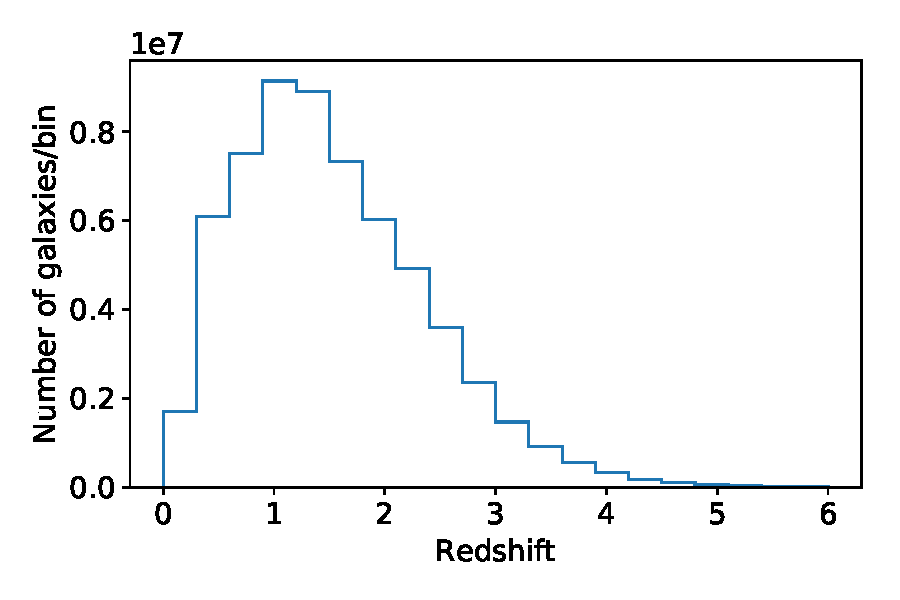
\includegraphics[width=0.9\columnwidth]{N_z_DC1.pdf}
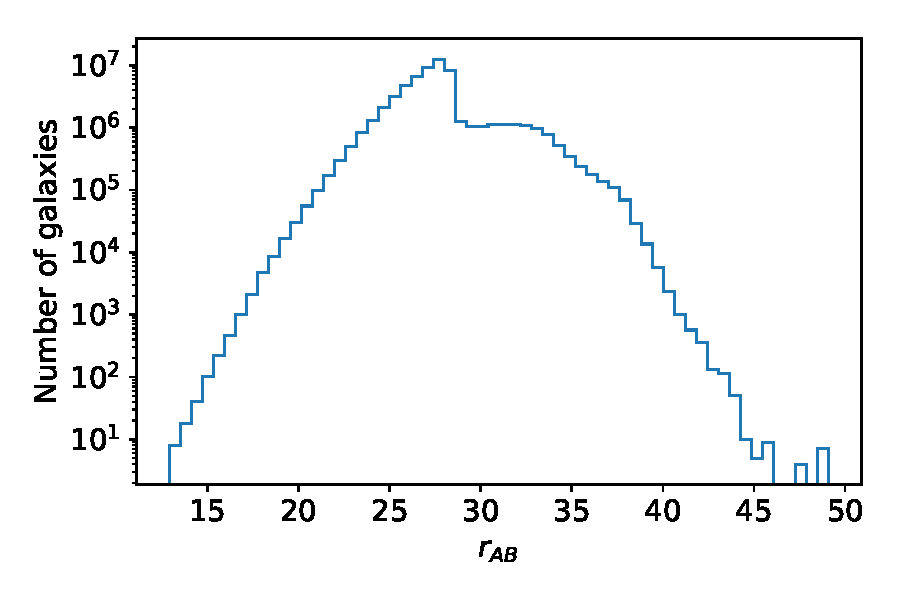
\includegraphics[width=0.9\columnwidth]{N_m_DC1.pdf}
\caption{Redshift (top) and magnitude (bottom) distribution for the galaxies used as inputs for DC1.}
\label{fig:catalog_plots}
\end{figure}

\begin{figure}
\centering
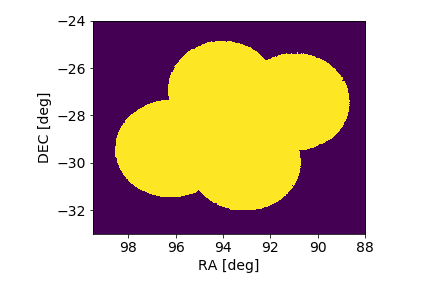
\includegraphics[width=0.9\columnwidth]{footprint.png}
\caption{Footprint of the DC1 dataset. We simulate 4 LSST full focal plane pointings which roughly corresponds to 40 square degrees.}
\label{fig:footprint}
\end{figure}

\section{Dithering strategy}
\label{sec:dithering}
\textcolor{red}{Please, Humna and/or Eric check this section.}

Different dithering strategies impact survey uniformity and systematic effects in photometric redshift surveys~\citep{2016ApJ...829...50A}. Simulating two different strategies is a beneficial check to determine the most effective strategy to mitigate systematic effects and yield better cosmological constraints. For this data challenge we use two different dithering strategies: the \textit{undithered} which points the telescope at the same position and orientation for all exposures in a given field; and the \textit{dithered} which consists in small random rotational and translational dithers for each pointing/exposure. This dithering strategy is stored in the OpSim\footnote{\url{https://www.lsst.org/scientists/simulations/opsim}} database presented in ref.~\citep{2016ApJ...829...50A}. However, with dithering, we might have some visits where part of the focal plane lies outside of our region of interest. We also simulated these visits, however, in order to save computational resources, we decided not to simulate the chips that lie outside of the region of interest.
\section{Image generation: pipeline}
\label{sec:image_generation_pipeline}
% ---------------------------------------------------------------------

The artificial generation of astronomical images is a complex and computationally demanding process. In the recent
years there is a big effort in the community in order to create software that allows more realistic and fast image
generation like \texttt{BALROG}~\citep{2016MNRAS.457..786S} or \texttt{UFIG}~\citep{2016ApJ...817...25B}. In our case, we model the input sources using imSim which uses \textsc{GalSim}~\citep{2015A&C....10..121R} as a library driven
by a LSST specific application. There are other approaches consisting in
running a full photon-shooting simulation using \textsc{PhoSim}~\citep{2015ApJS..218...14P}. \textcolor{red}{This approach will also be used in future Data Challenges. The former has a speed
advantage but the latter fully traces each photon coming from the sources through the atmosphere and the instrument,
increasing the level of realism with a fairly high computational cost. These two approaches can potentially allow us to focus on different systematic effects and science cases. -> Rewrite}

\subsection{imSim}
\label{sec:imsim_pipeline}

imSim follows the path of the fast image simulations in refs.~\citep{2016MNRAS.457..786S,2016ApJ...817...25B}.
imSim uses \textsc{GalSim}~\citep{2015A&C....10..121R} as a library to generate images that resemble LSST individual visits. Instead of the
planned two 15 seconds exposures planned~\citep{2008arXiv0805.2366I} we generate a single 30 seconds image to simplify the data handling.
We simulate each CCD of the focal plane individually but there are no instrumental effects nor variability in the optical model
across the focal plane except for the sky. We used an ESO sky model and the sky brightness values come from
OpSim~\citep{2014SPIE.9150E..15D}\footnote{We used the values at OpSim's run \texttt{minion\_1016}}. The PSF model that we use is a Gaussian for the system with a FWHM that depends on the airmass
\footnote{From LSST-20160 eqn. (4.1)} plus a Kolmogorov profile to model the atmosphere that is airmass dependent as well
\footnote{From LSST-20160 eqn. (4.2)}. The airmass model is taken from~\citep{1991PASP..103.1033K};
\begin{equation}
X = (1 - 0.96\sin{Z})^{-0.5},
\end{equation}
where $X$ is the airmass, and $Z$ the angular distance to the zenith.

In this simulation we generated three different types of objects: Stars which are modeled as PSF-like objects; galaxies, which are modeled as S\'{e}rsic profiles~\citep{1963BAAA....6...41S} (bulge plus disk) using
the parameters given by CatSim; and AGNs that are also modeled as very narrow Gaussian profiles. In this version of the catalog we decided
to not include variability in AGNs to simplify the analysis. The zeropoints are computed using the model presented at~\citep{2008arXiv0805.2366I} and the
throughputs at \url{https://github.com/lsst/throughputs} \textcolor{red}{David and I used the throughputs from the repo to compute these zeropoints. Should I add a table with them?}. We clip the objects at magnitude 10 to simulate saturation.

The final products of this pipeline are FITS images with information about the observing conditions. We generated more than 200,000 images in total (including both the \textit{dithered}, and \textit{undithered} fields). The average time to simulate each CCD is $\sim 4300$ seconds and the total production time was $\sim 270,000$ CPU-hours.

% ----------------------------------------------------------------------

%\subsection{PhoSim}
%\label{sec:phosim_pipeline}

%PhoSim is a complementary approach where we use the photon-shooting software \textsc{PhoSim} to create simulated images.
%\textcolor{red}{Describe PhoSim. PhoSim inputs and differences with imSim. What are we adding?}
% ----------------------------------------------------------------------
\subsection{Image processing pipeline}
\label{sec:image_processing_pipeline}

The outputs of these simulations are then processed using the LSST data management (DM) stack~\citep{2008arXiv0805.2366I,ScienceBook,WhitePaper,2017arXiv170506766B,2015arXiv151207914J} . This is an open
source high-performance data processing and analysis system intended for use in O/IR survey data. The code can be found at \url{dm.lsst.org} and \url{pipelines.lsst.io}. The raw, uncalibrated single exposures are used as inputs. The software performs the reduction, detection, deblending and measurement on individual visits and coadds producing the level 2 data products~\citep{2015arXiv151207914J}. Although it is still under development, most of the pieces already meet the science requirements. The DM stack provides calibrated images and source catalogs for the individual visits, and coadds stored in \texttt{FITS} files. In total, we detect and measure $\sim 10.6$ million objects with position, flux and shape information. We activated optional extensions for the pipeline to include \texttt{CMODEL} fluxes (see \cite{2017arXiv170506766B} for more details) and \texttt{HSM} shapes~\citep{2003MNRAS.343..459H,2005MNRAS.361.1287M}.

An example of a coadd image can be seen at \figref{coadd_example}.

\begin{figure}
\centering
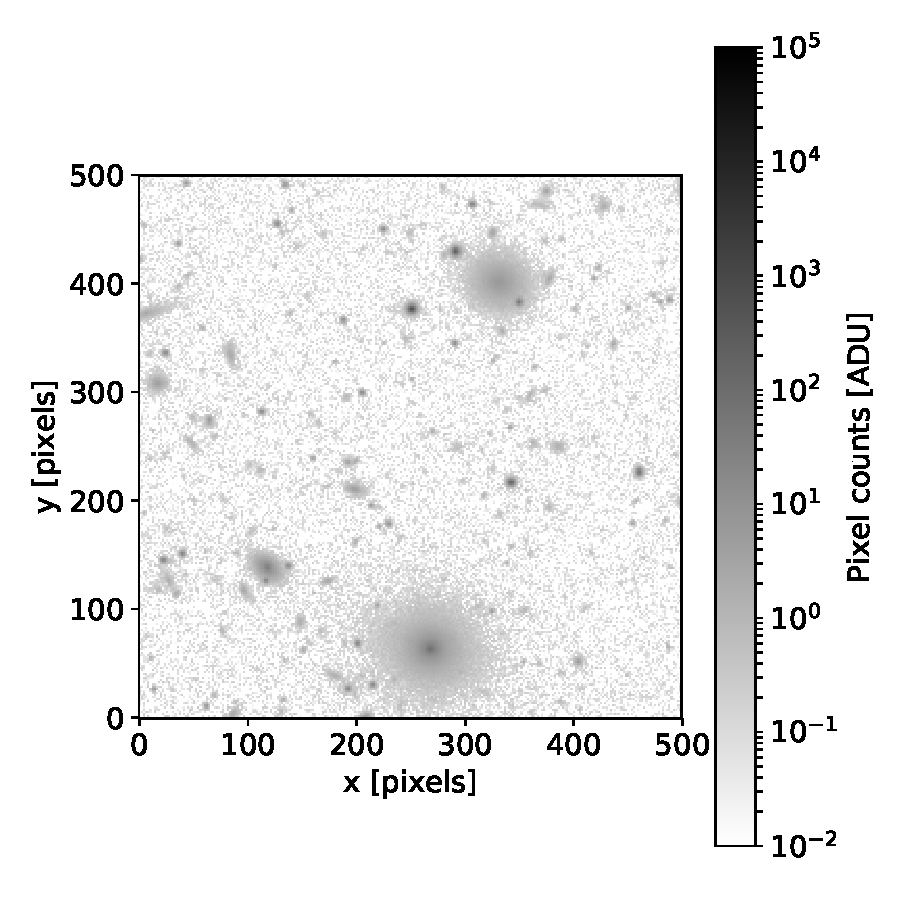
\includegraphics[width=0.9\columnwidth]{sample_coadd_DC1.pdf}
\caption{Example of a 500 $\times$ 500 pixel cutout from a full depth coadd. We can appreciate the large density of simulated objects.}
\label{fig:coadd_example}
\end{figure}

\section{Output catalogs and validation}
\label{sec:catalogs}

After being processed, the catalogs are accessible by DESC collaborators and stored at the National Energy Research Scientific Computing Center (NERSC)\footnote{\url{http://www.nersc.gov}}. We generate \texttt{pandas
dataframes}~\citep{mckinneypandas} and databases for each one of the coadds and input catalogs in order to be accessed by the collaborators and perform their own analyses. The output catalogs contain 10.6 million objects covering an area
of $\sim$ 43 deg$^{2}$. The catalogs include information about position, size, shape and magnitude for every object. They include several flags that give information about the presence of interpolated/saturated pixels in the objects or whether these objects are close to the edge of a CCD or not.

In order to check the level of realism and the accuracy of the processed catalogs we perform several quality assurance tests.

\subsection{Astrometry checks}
\label{sec:astrometry_checks}

Biases in astrometry can potentially affect both clustering and weak lensing measurements. These biases can have different origins: PSF mis-characterization, non corrected sensor effects, incorrect modeling of proper motion for the measured objects and presence of blended sources are among the most common sources.

We will follow two approaches to check the quality of the astrometric solutions that we obtained: an \textit{external} check comparing to the input \textit{truth} catalog; and an \textit{internal} check comparing different visits.

\subsubsection{External checks}
\label{sec:external_astrometry}

As we have already mentioned, one of the big advantages of using simulations is that we have access to the \textit{true} underlying information. We will use this information to check the precision of the astrometric measurements in single exposures
and co-adds. For these studies we will select stellar objects. In order to do so, we use the classifier included in the LSST software stack\footnote{To see more details about the classifier refer to section 4.9.10 at ~\citep{2017arXiv170506766B}} and choose objects with \texttt{base\_ClassificationExtendedness\_value==0}.
We also require that \texttt{deblend\_nChild==0} to ensure that the objects are completely deblended, i.e., they are primary sources. We match these objects to the stellar sources in the input catalog. In both cases we will use a \texttt{KDTree}~\citep{scikit-learn} to retrieve those objects in the input catalog that are in a radius of 0.2 arc-seconds (one pixel) of those detected in the output catalog and select the match that is closest in magnitude. We only consider sources which have a magnitude difference smaller than 0.02 magnitudes. We will discuss matching strategies in more detail at \secref{matching}.

We selected a representative single visit (visit number $270675$ for the imSim dithered run) and calculated the difference between the measured and the input positions. These are represented in \figref{astrometry_a}. We can see that both RA and Dec distributions are compatible with each other, meaning that there are no anisotropies in the detection, as expected from the inputs.
However, we find that the distributions are asymmetric and that the median is not zero. This effect is even more noticeable when we accumulate visits as in \figref{astrometry_b}, where we accumulated the results for 50 randomly selected visits of the imSim dithered run. This effect is also present in the undithered imSim run. We also checked the dependence the mean astrometric residual with the magnitude of the objects as shown in \figref{astrometry_b} where a mild bias for the brightest objects can be seen. This bias is smaller than 15 mas, much smaller than the resolution of the input N-body simulation. This means that the two point clustering statistics will not be affected by this bias. This bias arises from the fact that the objects in the images include proper motion, which is unaccounted for in our \textit{truth tables}.

\begin{figure}
  \centering
  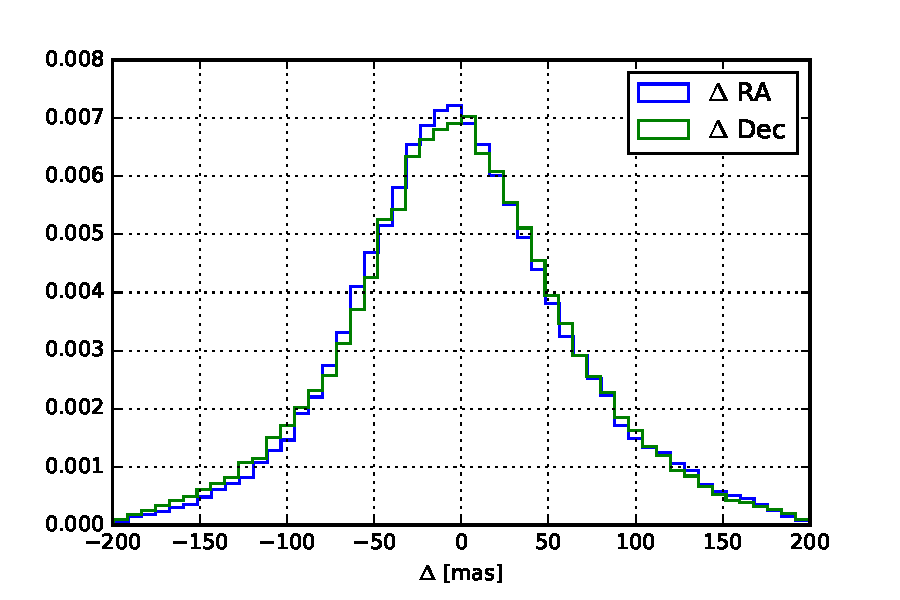
\includegraphics[width=0.45\textwidth]{astrometry_single_visit_imsim_dithered_hist}
  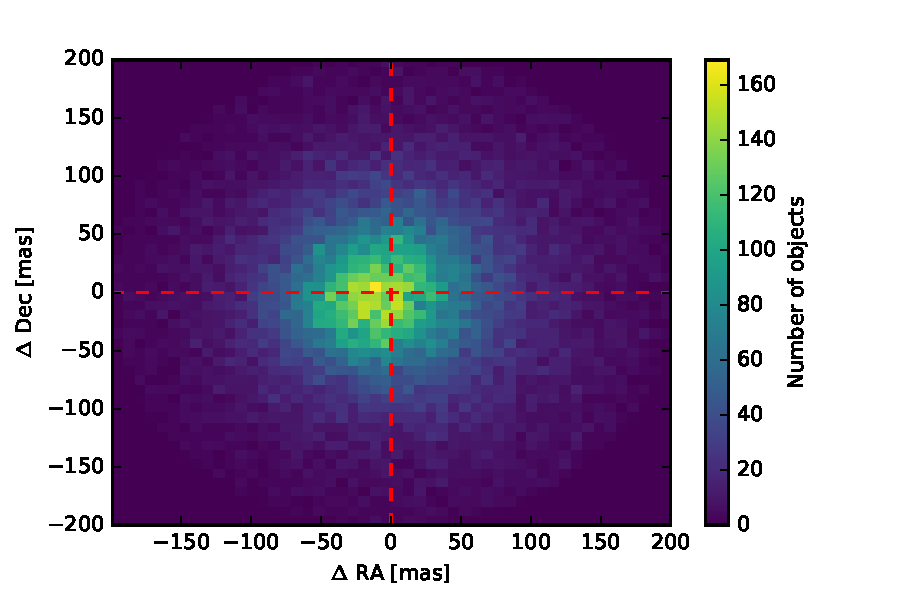
\includegraphics[width=0.45\textwidth]{astrometry_single_visit_imsim_dithered_hist2d}
  \caption{Left: Distribution of the difference $\Delta=X_{measured}-X_{input}$ in RA (blue) and Dec (green) coordinates. We cannot
  appreciate any differences between these, however we see that there is median is not at zero $\Delta_{median} \approx -2$ mas.
  The histograms are normalized such that the total sum of the counts is equal to one. Right: 2D histogram
  showing the bivariate distribution of the difference in RA (horizontal axis) and Dec (vertical axis). We selected one random representative
  exposure (visit number $270675$ for the imSim dithered run). The effect is similar for the undithered imSim run and for the PhoSim run.}
  \label{fig:astrometry_a}
\end{figure}

\begin{figure}
  \centering
  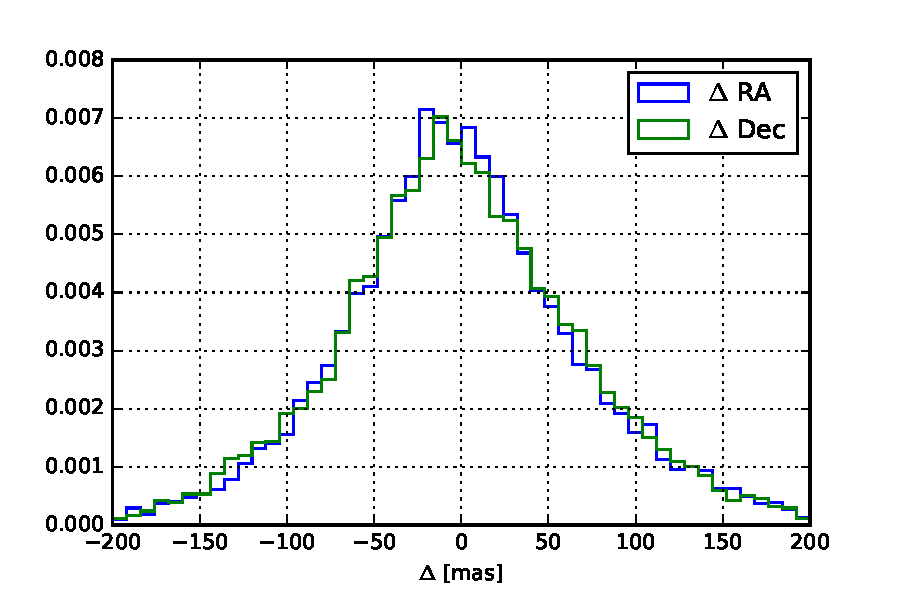
\includegraphics[width=0.3\textwidth]{astrometry_imsim_dithered_50visits}
  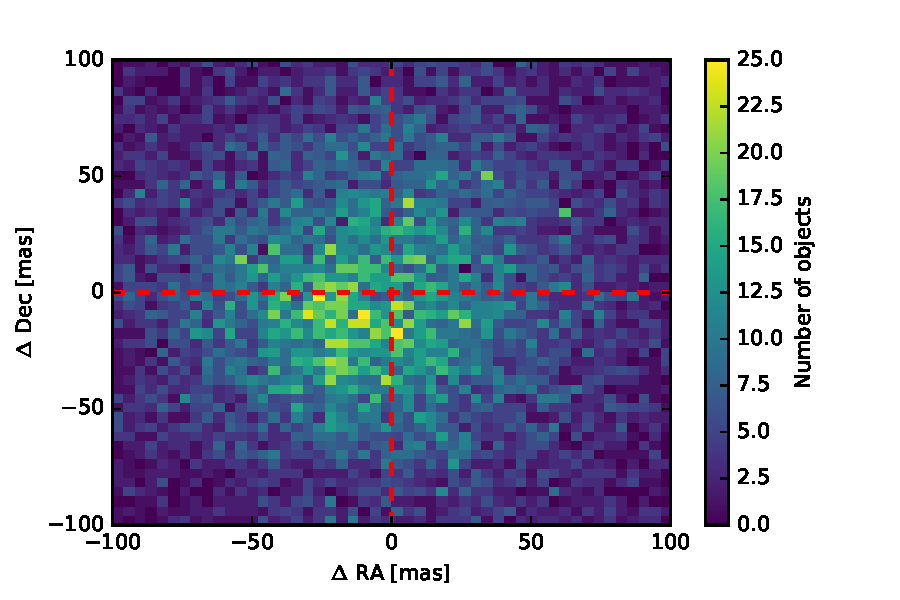
\includegraphics[width=0.3\textwidth]{astrometry_imsim_dithered_50visits_hist2d}
  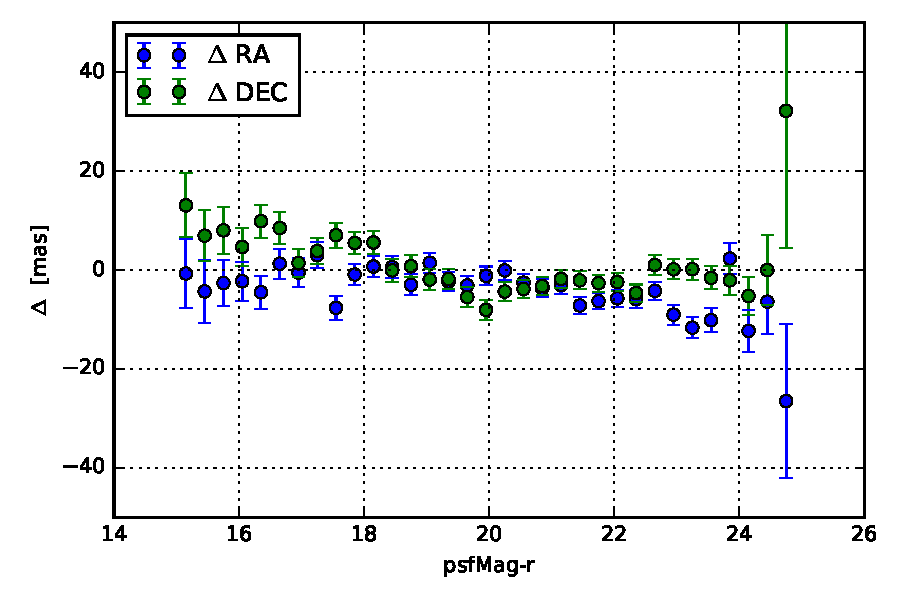
\includegraphics[width=0.3\textwidth]{astrometry_vs_mag_imsim_50_visits}
  \caption{Left: Distribution of the difference $\Delta=X_{measured}-X_{input}$ in RA (blue) and Dec (green) coordinates as in
  \figref{astrometry_a} but accumulating the results for 50 randomly selected visits from the imSim dithered run. Middle: 2D histogram
  showing the bivariate distribution of the difference in RA (horizontal axis) and Dec (vertical axis). Right: Mean astrometric residual
  as a function of magnitude for RA (blue) and Dec (green). These distributions are similar for the undithered imSim run and for the PhoSim run.}
  \label{fig:astrometry_b}
\end{figure}

We also wanted to check if there is a preferred orientation for the differences between the input and output position in a single visit. Using the same visit as before we show the astrometric residuals in \figref{astrometry_c}. In this Figure we can see that the astrometric residuals do not show any noticeable structure and appear to be mostly random with the largest contributions close to the CCD edges.

\begin{figure}
  \centering
  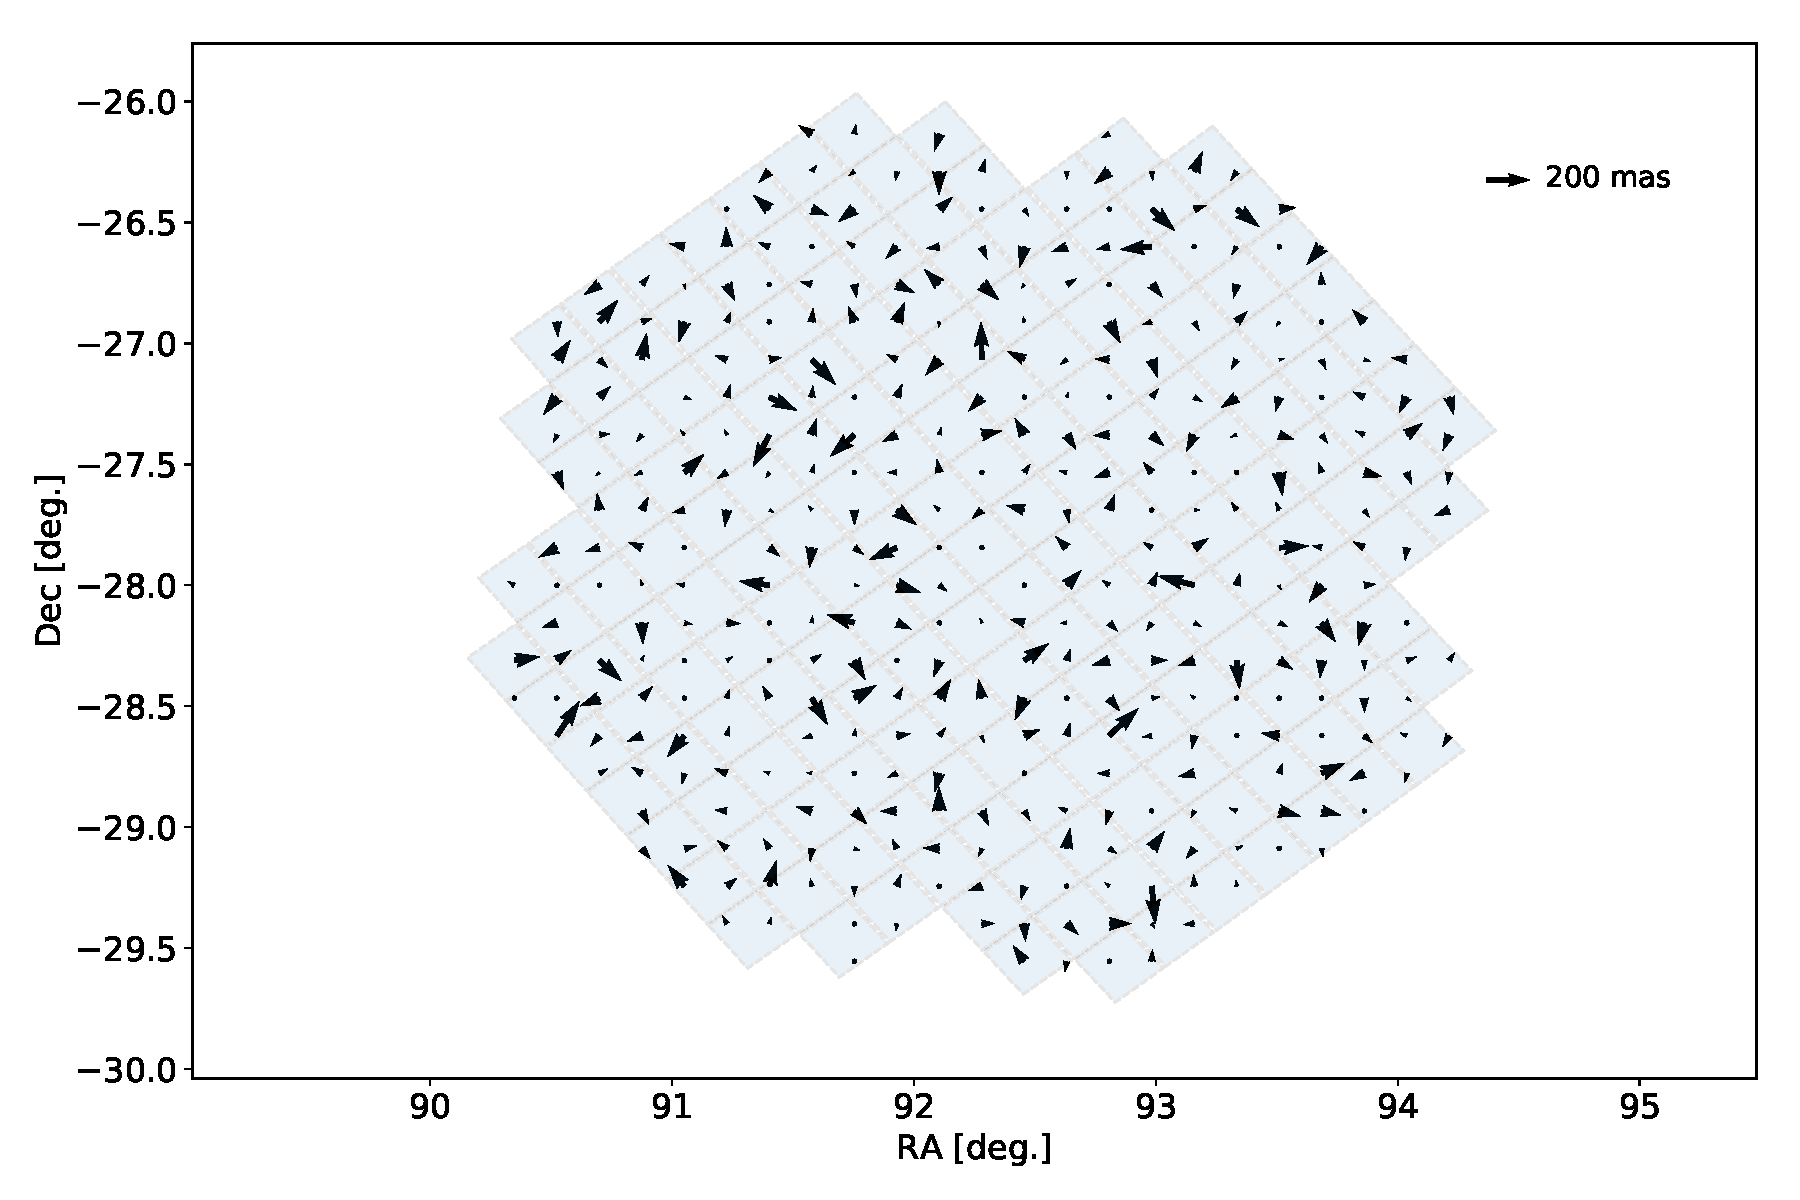
\includegraphics[width=0.45\textwidth]{astrometry_imsim_dithered_interp}
  \caption{Astrometic residuals measured in visit $270675$ from the imSim dithered run. The light blue squares represent the CCD chips in
  the LSST focal plane. The base of the arrow is on the input matched object. The arrows have been re-scaled 10,000 for visualization purposes.}
  \label{fig:astrometry_c}
\end{figure}


\subsubsection{Internal checks}
\label{sec:internal_astrometry}

Another important test is to ensure the internal consistency of the astrometric solutions between different exposures. To do that we selected
a small region of the co-added area (\textit{patch}) and compared the positions of the objects detected in the co-add
image with the positions of objects detected in individual exposures that overlap with that patch.

In particular, we randomly chose 10 catalogs from individual exposures and looked for objects that fulfilled the following criteria:
\begin{itemize}
  \item \texttt{deblend\_nChild==0}, this means that the object has been completely deblended (it is a primary match).
  \item \texttt{base\_PixelFlags\_flag\_edge==0}, which means that the object is not close to an edge.
  \item \texttt{base\_PixelFlags\_flag\_interpolatedCenter==0}, the object does not have any interpolated pixels in its center.
\end{itemize}

Note that in this case we are not requiring the objects to be classified as stars (we are omitting the cut in
\texttt{base\_ClassificationExtendedness\_value}) but we are adding some cuts to ensure that the objects were properly measured. Once
we perform our selection, the next step is to match the objects in the different exposures. To do so we use the matching algorithm
included in the LSST software stack\textcolor{red}{Reference?} and calculate the mean of the difference between the position of each source
in the co-add, $X_{coadd,i}$ and the position of the matched object in each of the exposures where it has been detected, $X_{visit_{j},i}$
for $j \in [1,10]$, i.e,

\begin{equation}
  \Delta = \langle X_{coadd,i} - X_{visit_{j},i} \rangle
\end{equation}
we only consider sources that have been detected in at least 5 exposures. The resulting distribution is shown in \figref{astrometry_internal}
where we see that is noticeably narrower than those shown in \figref{astrometry_a} and \figref{astrometry_b} and no apparent bias is found showing
that the processing is consistent.

\begin{figure}
  \centering
  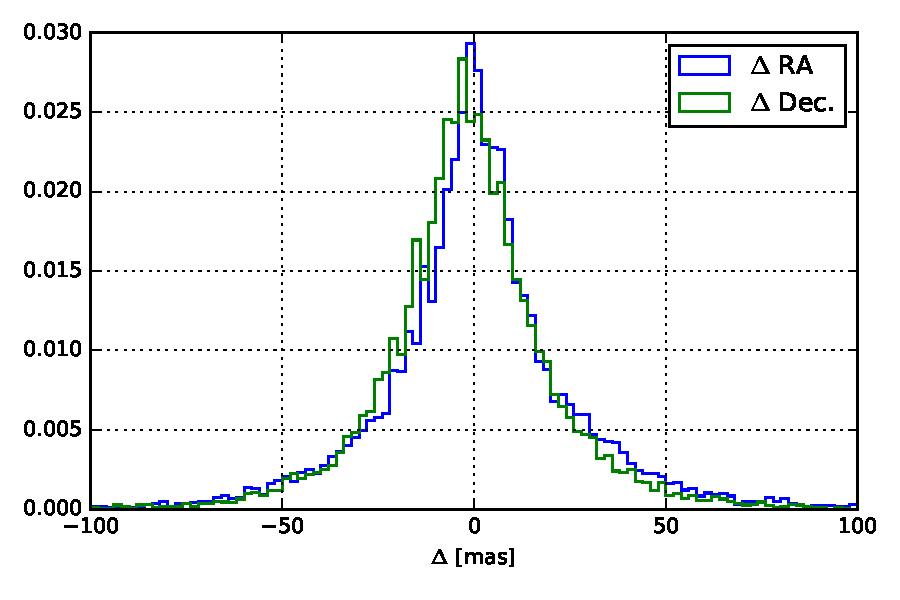
\includegraphics[width=0.45\textwidth]{astrometry_internal_10visits_imsim_undithered}
  \caption{Distribution of the mean difference in position (RA:blue, Dec:green) between the coadd and the different individual exposures
  where each source has been detected.}
  \label{fig:astrometry_internal}
\end{figure}

\subsection{Photometry checks}
\label{sec:photometry_checks}

As we did in previous sections we perform two different tests to assess the quality of our simulations: first we compare our output catalogs to the inputs, and second we check the consistency between different visits for the same objects.

\subsubsection{External checks}
\label{sec:external_photometry}

We want to analyze the accuracy of the magnitude measurement comparing the input catalog with the output catalog. This process not only checks
the accuracy of the measurement pipeline, but it also tests the quality and level of realism of the image generation pipeline.
For these external checks we use again the same 50 randomly selected visits as we did in the previous section to check the astrometric residuals.
To study the photometric residuals we change slightly the matching strategy from previous sections. In this case we eliminate the threshold
in magnitude difference so, we just look for the input source that is closest in magnitude in a 0.2 arc-seconds radius around each detected
source. In \figref{photometry_a} we can see the distribution of the photometric residuals. We see that this distribution gets wider as we go
fainter (as expected) and that the 0.02 magnitude selection cut was a good proxy to ensure that we account for most sources properly matched.

\begin{figure}
  \centering
  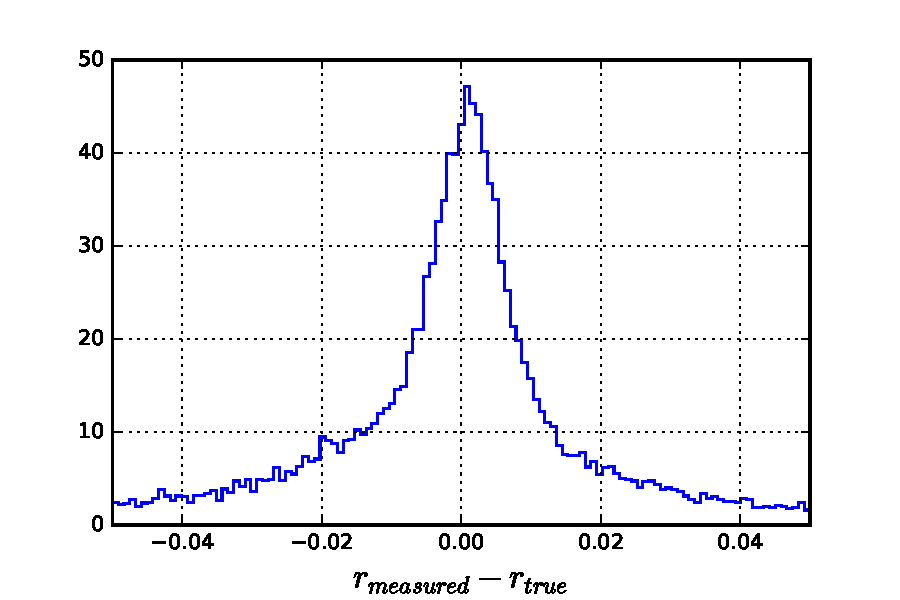
\includegraphics[width=0.45\textwidth]{photometry_imsim_dithered_50visits_hist}
  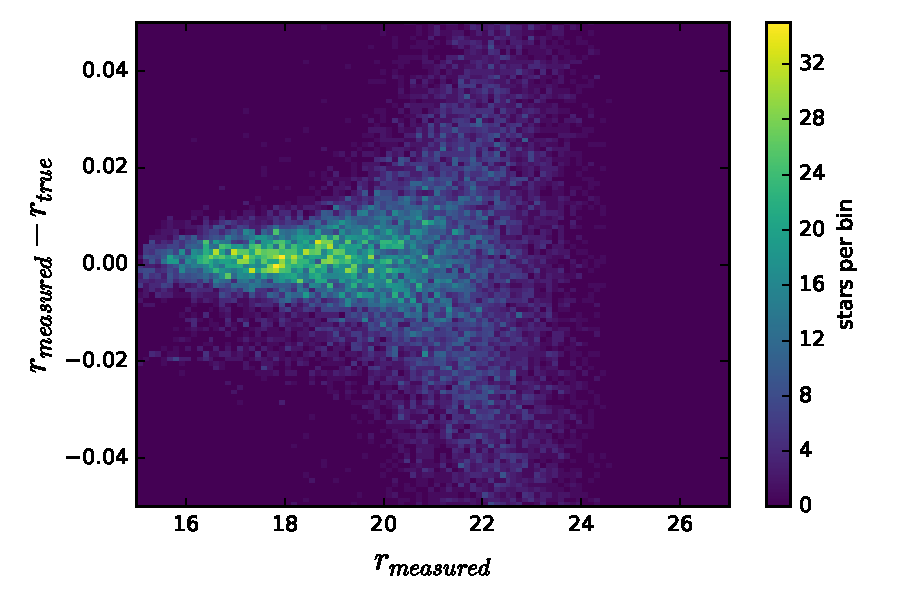
\includegraphics[width=0.45\textwidth]{photometry_imsim_dithered_50visits}
  \caption{Left: Distribution of magnitude difference between the input and output catalogs.
  Right: Difference magnitude between input and output catalogs as a function of the measured magnitude. We considered 50 visits
  randomly selected from the imSim dithered run. We find similar results for the imSim undithered run and for the PhoSim run.}
  \label{fig:photometry_a}
\end{figure}

\subsubsection{Internal checks}
\label{sec:internal_photometry}

We also checked the consistency of the photometry between different exposures. Using the same approach and sample presented in
\secref{internal_astrometry} we compared the mean difference between the coadded source and 10 random single-visit images. In
principle, we would expect that some objects will show differences between different epochs due to their intrinsic variability, however,
these effects are not found in the inputs of the simulation for any of the objects, thus, the differences between different epochs will come mainly
from statistical fluctuations and different observing conditions. The results from these checks can be seen in \figref{internal_photometry_a}.

\begin{figure}
  \centering
  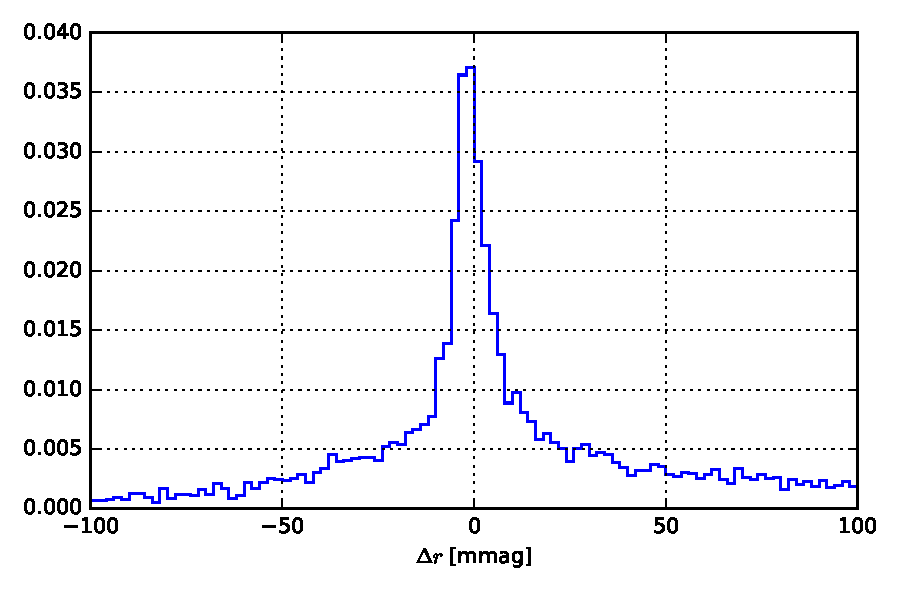
\includegraphics[width=0.45\textwidth]{photometry_internal_10visits_imsim_undithered}
  \caption{Distribution of the mean difference in magnitude between the coadd and the different individual exposures
  where each source has been detected. The mean of the distribution is consistent with zero.}
  \label{fig:internal_photometry_a}
\end{figure}

In this figure we can see that the mean of the distribution is compatible with zero and that most sources have a magnitude difference lower
than 25 mmag given the narrow peak. The presence of long tails are likely due to blends and mismatching or artifacts.

\subsection{PSF checks}
\label{sec:psf_checks}

In order to ensure the accuracy of shape measurements a robust and accurate estimation of the PSF is required. In the case of imSim, we have
a perfectly known input PSF that only depends on the airmass at the time of observation. We can check if the measurement pipeline can reconstruct
the PSF and at which level of precision. To do that, we select 200 visits randomly, retrieve the measured PSF using the pipeline, and compare this
to the input model given the observing conditions and compute the residual. We obtain the residual depicted in \figref{psf_residual}, where we can see that the PSF is recovered correctly with a high level of precision and accuracy.The very small residual in the center and the tails are dominated by noise.

\begin{figure}
\centering
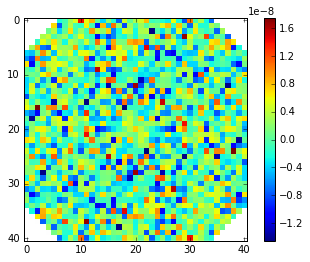
\includegraphics[width=0.9\columnwidth]{psf_residual.png}
\caption{Average difference between the input PSF model (41$\times$41 pixels, normalized to unity) and the measured PSF (with the same normalization) for 200 visits.}
\label{fig:psf_residual}
\end{figure}
\section{Analysis of the simulated dataset}
\label{sec:analysis}
In this section we are going to analyze the clustering properties of our output catalog from the end-to-end pipeline and compare to the input catalog.

\subsection{Matching input and output catalogs}
\label{sec:matching}

Potentially, in end-to-end simulations, one can trace back each measured photon to its corresponding source in order to characterize the measurement process. However, this is not always possible for several reasons. For example, a simple solution could be storing each postage stamp for the different sources in different exposures. The problem with this approach is that it creates a large overhead in an already big dataset. Generating efficient strategies to perform this bookkeeping and connecting input and output catalogs is then, an important research topic for these kinds of end-to-end simulations. 

The simplest way to connect two catalogs is by using the positions of the objects in the sky. This approach has been extensively used in the literature and performs reasonably well when blending is low, since the probability of confusing two objects is small. However, when blending is high, this approach might be not enough and matching other quantities like flux or shape can become useful, even though these can introduce some subtleties, an example being, how to weigh positions versus fluxes (and/or shapes) and whether or not we should consider the correlations between the two.

We compare two different matching strategies: simple spatial matching, where we match the find the objects in the truth catalog closest to the detected objects; and spatial matching including magnitude matching, where for each detected object we find which objects from the input catalog lie within one pixel radius ($0.2 \arcsec$). After this we select the object that is closest in magnitude, as long as the difference in magnitude is less than a certain threshold. In our case, we arbitrarily chose $0.5$. If any of these conditions are not fulfilled, then the object is thrown away.

In the former approach all detected objects are matched to an object in the input catalog and, in principle, the two point statistics should be preserved between these two catalogs. However, in the latter approach, we can potentially bias the results since we are throwing away galaxies where the accuracy in the magnitude measurement is low, regardless of the precision. To compare both approaches we check the possible biases in the measured magnitude $\Delta$mag = mag$_{meas} - $mag$_{true}$. In \figref{matching_comparison} we can see that spatial matching is enough to get a good match in magnitude as evidenced by the median value of $\Delta$mag compared with the spatial+magnitude matching. This figure also shows that spatial matching is more affected by the presence of outliers than the spatial+magnitude matching, as expected by the clipping performed on the latter. The evolution of the mean and median $\Delta$mag with the magnitude evidences that brighter objects with magnitudes $\sim 18-21$ appear usually brighter and, on the other hand, fainter objects with magnitudes $\sim 23-25$ appear dimmer, this is likely a consequence of the deblender assigning a larger flux to the brightest members of the blend, while the fainter members seems to be losing flux. Finally, since for the faintest end (mag $\sim 26$) we can only detect those that appear brighter than they actually are and, thus, there is significant negative value for the median and mean $\Delta$mag.

\begin{figure}
\centering
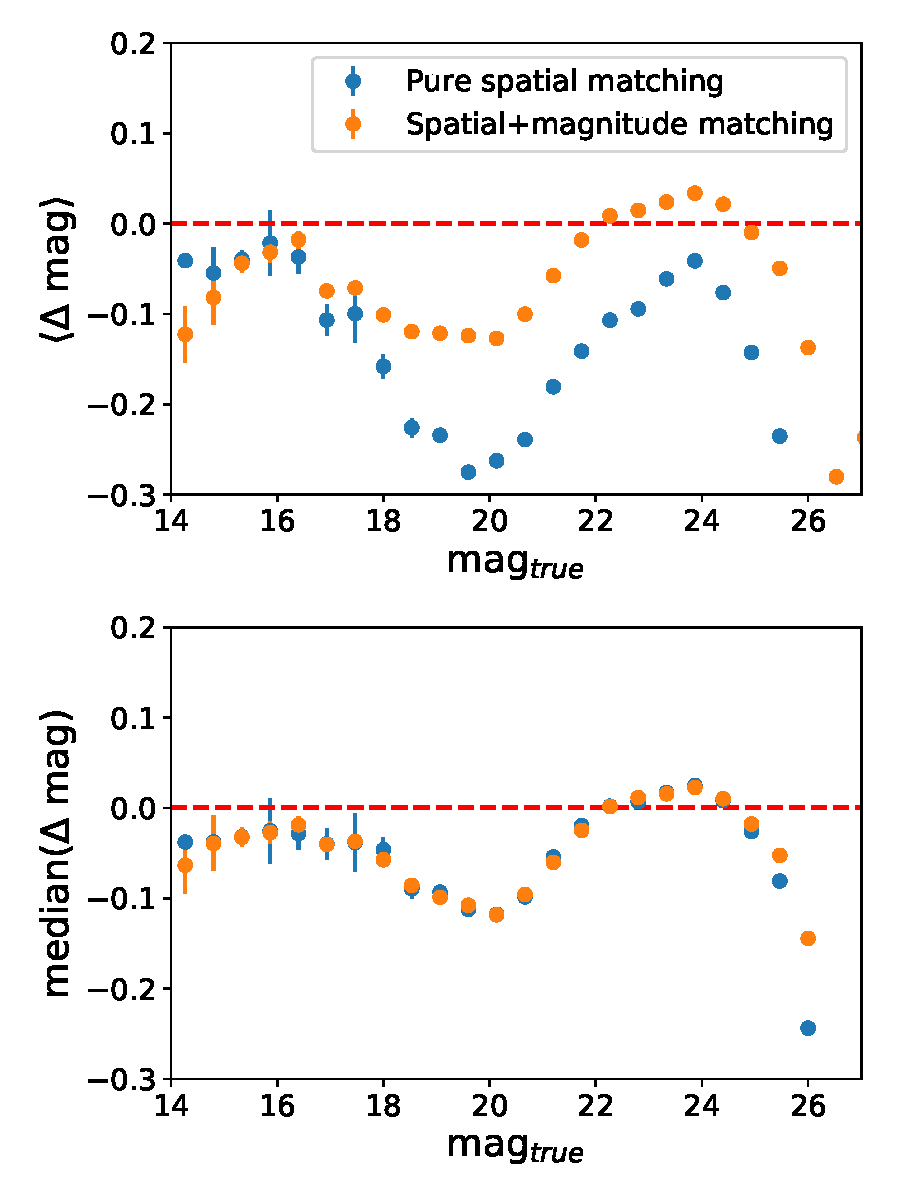
\includegraphics[width=0.9\columnwidth]{matching_comparison_galaxies.pdf}
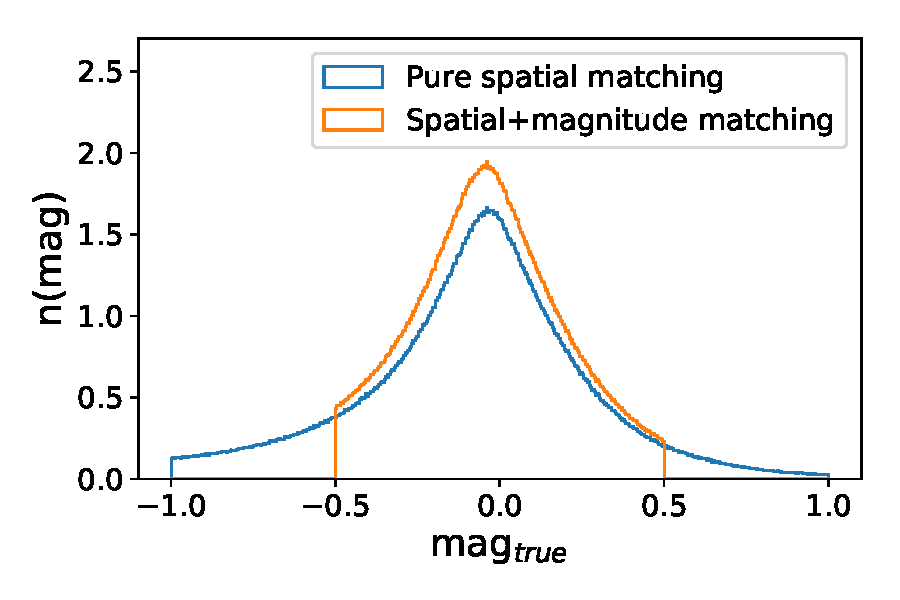
\includegraphics[width=0.9\columnwidth]{mag_hist_total.pdf}
\caption{Mean (top), and median (middle) of $\Delta$mag as a function of the true magnitude, with pure spatial matching (blue) and spatial+magnitude matching (orange). Bottom: Histogram of $\Delta$ mag.}
\label{fig:matching_comparison}
\end{figure}

We also compared the power-spectra of the detected objects and the matched input objects in \figref{matching_cls}. In this figure we can see that the spatial matching recovers really well the power-spectrum, with some wiggling at very low scales due to mismatches and small differences in position between the detected and the input catalogs. In the case of spatial+magnitude matching, we see that the power for the matched catalog is consistently lower. This is due to the galaxies that are detected but not matched to any object in the true catalog, since this effect disappears when we just consider the objects that have been matched.

\begin{figure}
\centering
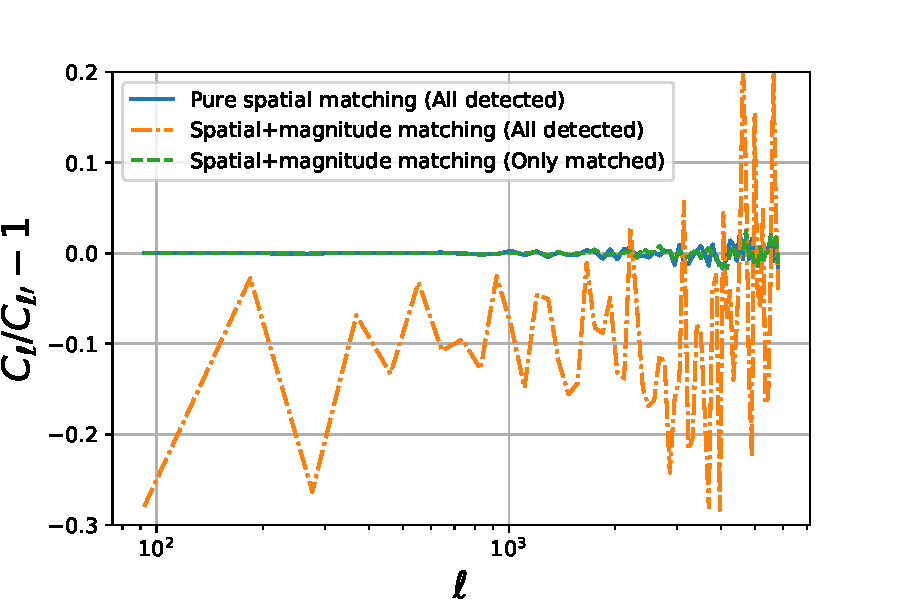
\includegraphics[width=0.9\columnwidth]{cl_comparison_matching.pdf}
\caption{Relative difference between the power-spectrum measured for the detected objects and the matched objects in the input catalog with spatial matching compared to all detected objects (blue, solid line), spatial+magnitude matching compared to all detected objects (orange, dash dotted line), and spatial+magnitude matching compared to matched objects using this schema (green dashed line).}
\label{fig:matching_cls}
\end{figure}
 
The problem with these matching techniques is the lack of very small scale information, and details about blended objects and groups, therefore, for analyses involving blending and/or very small scale information, different approaches should be considered. 
 
% ----------------------------------------------------------------------

\subsection{Generating depth maps}
\label{sec:masking}

In order to estimate the depth in the coadd catalogs we select the stars by using \texttt{base\_ClassificationExtendedness\_value==0}. This ensures selecting
PSF-like objects. After this, we have two different approaches:

\begin{enumerate}
\item In the first approach we generate a HEALPix\footnote{\url{http://healpix.sf.net}}~\citep{2005ApJ...622..759G} map containing the PSF-like objects detected with a signal-to-noise ratio (SNR) higher or equal than 5 (\texttt{base\_PsfFlux\_flux/base\_PsfFlux\_fluxSigma>=5}), and we assign to each pixel the value of the
dimmest object contained in it.
\item The second procedure also generates a HEALPix~\citep{2005ApJ...622..759G} map containing the PSF-like objects. Then in each pixel, we compute the median SNR as a function of the magnitude and get the magnitude at which SNR is the closest to 5.
\end{enumerate}

These two procedures yield very similar results (within $\sim 4\%$) as it can be seen in \figref{depth_comparison}. We checked that the maps built selecting galaxies instead of stars are compatible as well. We will select our footprint according to the depth map using the second methodology which can be seen in \figref{depth_maps}.

\begin{figure}
\centering
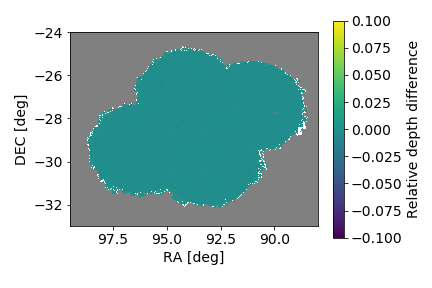
\includegraphics[width=0.9\columnwidth]{dithered_difference.png}
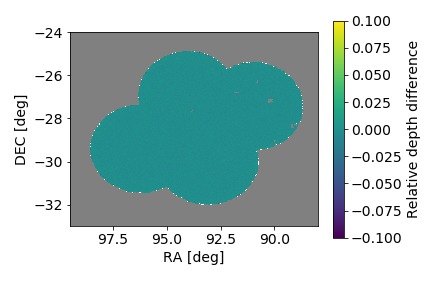
\includegraphics[width=0.9\columnwidth]{undithered_difference.png}
\caption{Relative difference between the depth calculated using the two methods presented in the text for the dithered (top) and undithered (bottom) fields.}
\label{fig:depth_comparison}
\end{figure}

\begin{figure}
\centering
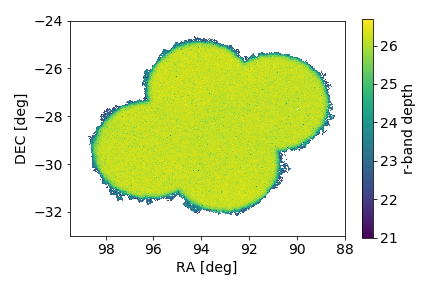
\includegraphics[width=0.9\columnwidth]{dithered_depth.png}
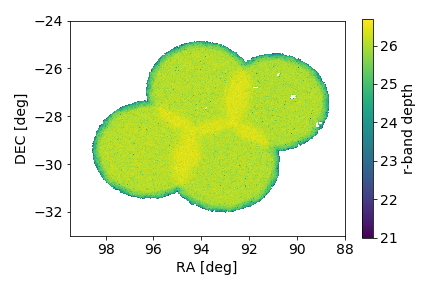
\includegraphics[width=0.9\columnwidth]{undithered_depth.png}
\caption{5-$\sigma$ depth for the dithered (top) and undithered (bottom) fields.}
\label{fig:depth_maps}
\end{figure}

\subsection{Bright objects masking and data selection}

Bright objects produce significant effects in the image that affects the detection and measurement of neighboring objects. Some examples of the effect of these objects are: saturation of the CCD, large diffraction spikes, obscuration of neighboring sources, etc. Thus, masking a region around these sources makes a more complicated footprint but greatly simplifies the analysis of systematic effects. In order to evaluate the effect of this sources, we use the stars from the input catalog, we divide them in different magnitude bins, and we count the detected objects in a given radius. The main problem with this methodology is that the points are correlated, the number of stars in an aperture of radius $\theta_{1} > \theta_{0}$, depends on the number of stars on the aperture with radius $\theta_{0}$. Therefore, it is better to use a differential measurement and this is what we do in \figref{galdens_derivative}. We can see that there is an excess of sources at distances lower than 10 arcseconds for the brightest stars. This is mainly due to the existence of fake sources around these bright objects. The brighter sources also have a larger noise, the DM deblender models the brightest source and subtracts this model looking for fainter sources that can be blended together with it. However, sometimes there are large noise peaks that have not been subtracted. These large noise peaks are detected in later stages as individual (point-like) sources giving as a result these fake sources. However, we do not see any obscuration present at the scales that we are interested (1 arcmin and higher) so it seems that no masking is required but we need to select the objects for our analysis carefully.

\begin{figure}
\centering
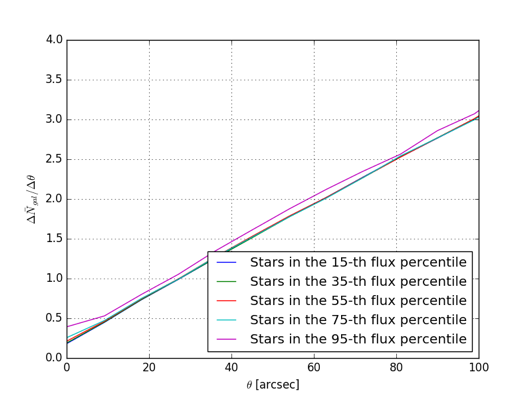
\includegraphics[width=0.9\columnwidth]{dngal_dtheta.png}
\caption{Mean increment in the number of detected objects around stars in the 95th flux percentile (magenta), the 75th percentile (cyan), the 55th percentile (red), the 35th percentile (green) and the 15th percentile (blue). We see that for the brightest percentiles there is no obscuration present but a overdensity of targets. These are mainly noise peaks identified as point sources.}
\label{fig:galdens_derivative}
\end{figure}

We checked the detection efficiency of galaxies in our sample. In order to do so we selected galaxies in the catalog using the variable \texttt{base\_ClassificationExtendedness\_value} as a star/galaxy separator as in ref.~\citep{2017arXiv170506766B}. Objects where this variable is 1 are more likely to be galaxies, whereas the objects where it is 0 are more likely to be stars. We also made some quality cuts by selecting the objects with \texttt{detect\_isPrimary==True}. This ensures that the object has been fully deblended and that the detection was not close to the edge of a coadded image. The results can be seen in \figref{completeness} where we computed the ratio of detected objects classified as galaxies and the input number of galaxies, $\varepsilon$ as a function of magnitude. We checked this ratio for both the dithered and undithered catalogs and in pixels where the depths were higher than 25.7 and 26.25. We used \texttt{CMODEL\_MAG} as the reference magnitude for the detected objects and the true magnitude for the input galaxies.

\begin{figure}
\centering
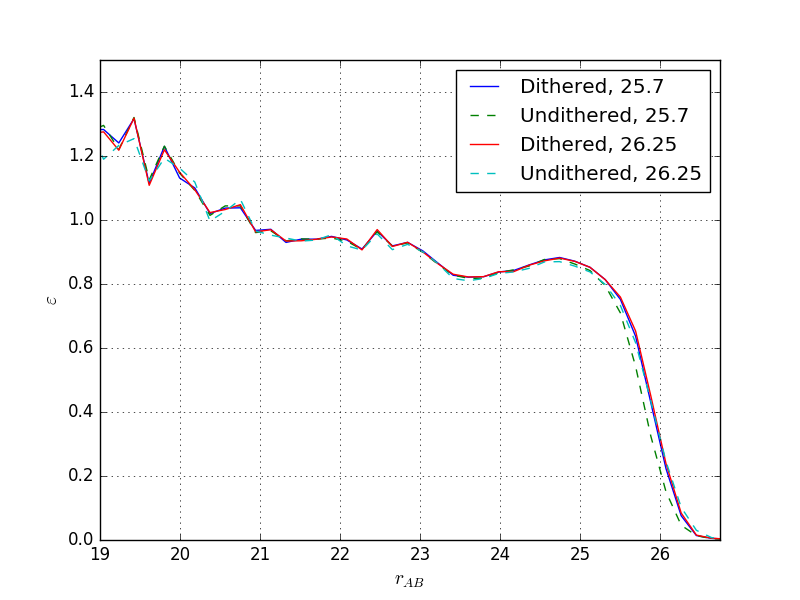
\includegraphics[width=0.9\columnwidth]{completeness.png}
\caption{Number of detected objects classified as galaxies divided by the number input galaxies as a function of magnitude. We see that the detection efficiency is larger than 80\% for the most part and a considerable fraction of objects with magnitude lower than 20 are being misclassified.}
\label{fig:completeness}
\end{figure}

Looking at \figref{completeness} it seems that selecting galaxies with \texttt{base\_ClassificationExtendedness\_value==1}, \texttt{detect\_isPrimary==True} and \texttt{CMODEL\_MAG $>$ 21} is enough to get rid of most potential problems with fake detections. We confirmed this by performing visual inspection on the images. We noticed that fake sources happen close to very bright objects. On top of that, it seems that selecting \texttt{CMODEL\_MAG $<$ 25.3} ensures good level of completeness ($\sim 80\%$). Uniformity is ensured by selecting the galaxies that lie within HEALPixels where the depth is greater or equal than 25.3. After these selection cuts we end up with 4.4 million galaxies for the dithered field and 4.3 for the undithered field. 
% ----------------------------------------------------------------------

\subsection{Clustering results}
\label{sec:results}

In this section we analyze the two point clustering statistics for both the dithered and undithered catalogs in real and harmonic space and check the consistency between the input and measured observables. When comparing the input and output catalogs some subtleties arise. Let us think of a galaxy that has been measured with magnitude $m_{meas}$ and with true magnitude $m_{true}$ and we choose a magnitude threshold $m_{threshold}$ to define the sample of interest. If the luminosity function were flat, and assuming that the errors in magnitude are symmetric (which is not true) we would have as many objects with $m_{meas}<m_{threshold}$, but $m_{true}>m_{threshold}$ as objects with $m_{meas}>m_{threshold}$ but $m_{true}<m_{threshold}$, and this wouldn't change very much the clustering properties of our sample and we could just compare directly the samples using the magnitude threshold in true magnitude and measured magnitude. However, this is not the case, given that the luminosity function is a growing function with magnitude, we expect more objects with $m_{meas}<m_{threshold}$, but $m_{true}>m_{threshold}$ than objects with $m_{meas}>m_{threshold}$ and $m_{true}<m_{threshold}$. So, in our measured sample we have more galaxies than in the sample selected with the true magnitude with the same magnitude threshold, making our selection wider, and therefore, reducing the total power.
\subsection{2-point correlation function}
Using the samples presented in previous sections, we measure the 2-point correlation function using the package \texttt{TreeCorr}~\citep{2004MNRAS.352..338J} with the Landy \& Szalay estimator~\citep{1993ApJ...412...64L}.

\begin{equation}
w(\theta) = \frac{DD - 2 DR + RR}{RR}
\end{equation} 
where $DD, DR$, and $RR$ are the number of pairs of objects taking from the data $D$ or the random catalog $R$ that covers the footprint. We use 30 angular log-spaced bins between $\theta=0.0001^{\circ}$ and $\theta=10^{\circ}$. The number of bins has been chosen so that the resulting covariance matrix is nearly diagonal. The covariance matrices are calculated using the delete-one jackknife technique~\citep{Shao:1986:DJB,2009MNRAS.396...19N}. We divide the footprint in $N_{JK}=100$ regions. These regions are defined using the K-means algorithm from the package \texttt{kmeans\_radec}\footnote{\url{https://github.com/esheldon/kmeans\_radec}}. The covariance matrix is then computed as
\begin{equation}
\mathrm{Cov}_{JK}(\theta_{i},\theta_{j})=\frac{N_{JK}-1}{N_{JK}}\sum_{k=1}^{N_{JK}}\Delta w_{k}(\theta_{i}) \Delta w_{k}(\theta_{j})
\end{equation}
\begin{equation}
\Delta w_{k}(\theta_{i}) = w_{k}(\theta_{i})-\bar{w}(\theta_{i})
\end{equation}
Where $w_{k}(\theta_{i})$ is the value of the correlation function when deleting the $k$-th region at the scale $\theta_{i}$, and $\bar{w}(\theta_{i})$ is the average correlation function at that same scale. We compute the correlation function on the dithered and undithered catalogs using their respective footprints, and we compare with the predicted correlation function given the $N(z)$ obtained by the spatial matching presented in previous sections, and using \texttt{CCL}\footnote{https://github.com/LSSTDESC/CCL}~\citep{CCL}. The results can be seen at \figref{2pt_corr}. 

\begin{figure}
\centering
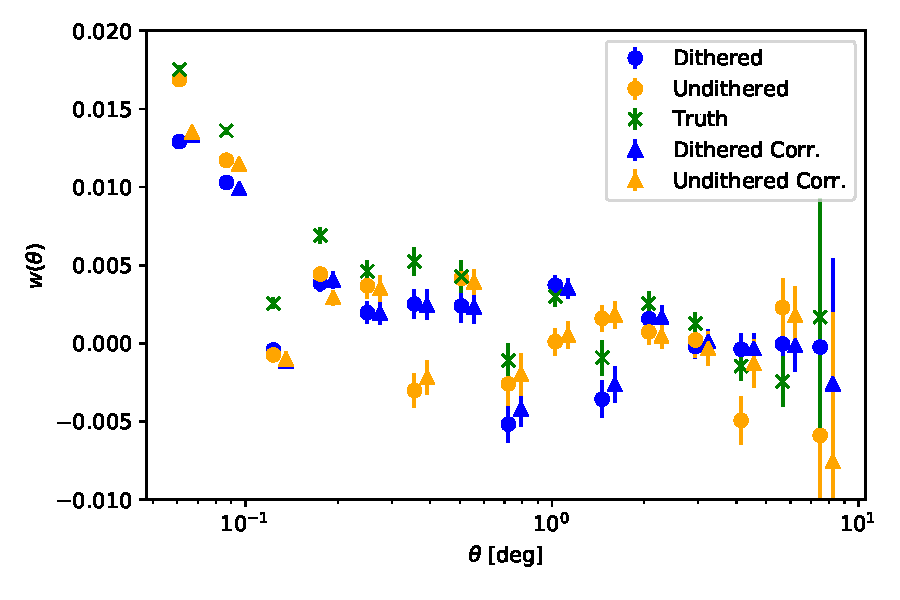
\includegraphics[width=0.9\columnwidth]{w_comp_corr25p3.pdf}
\caption{Results for the two-point correlation function in the input (green), dithered (blue) and undithered (orange) datasets. We can see that after the correction (triangles) for the systematic effects the agreement is better than without the correction (circles) between the input and output data especially for the undithered case (for the dithered case the corrections are negligible).} 
\label{fig:2pt_corr}
\end{figure}

%We also show the correlation matrix,
%\begin{equation}
%\mathrm{Corr}_{ij}=\frac{\mathrm{Cov}_{ij}}{\sqrt{\mathrm{Cov}_{ii}\mathrm{Cov}_{jj}}}
%\end{equation}
%in \figref{2pt_cov} where we can see that in both cases the matrices are almost diagonal.
%\begin{figure}
%\centering
%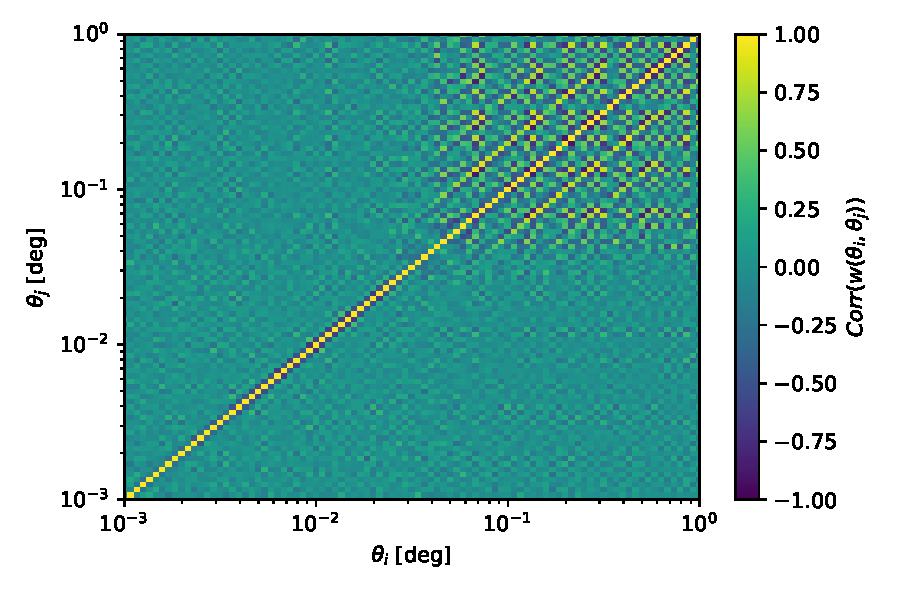
\includegraphics[width=0.9\columnwidth]{correlation_matrix_dithered_25p3_v2.pdf}
%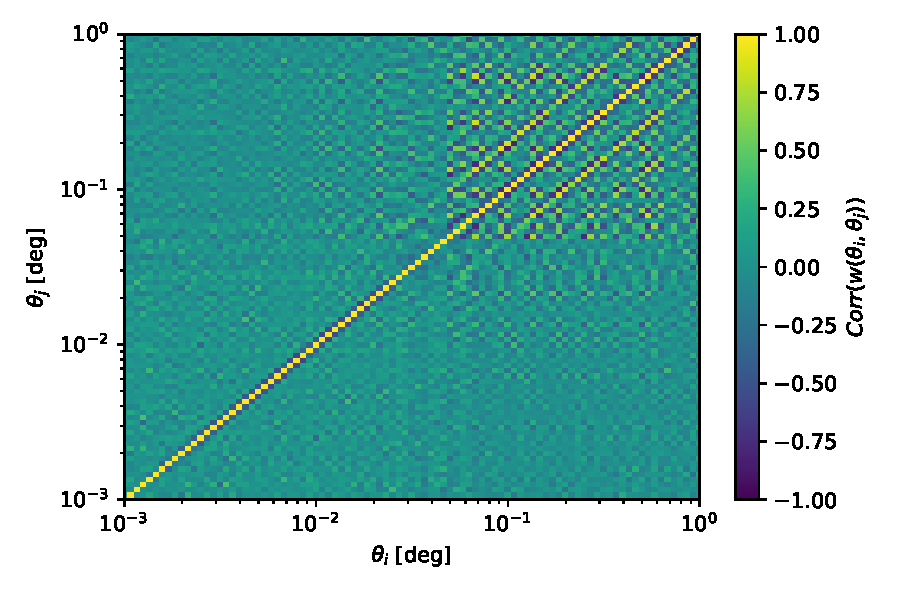
\includegraphics[width=0.9\columnwidth]{correlation_matrix_undithered_25p3_v2.pdf}
%\caption{Correlation matrices for the dithered (top) and undithered catalogs (bottom).}
%\label{fig:2pt_cov}
%\end{figure}
\subsubsection{Angular power spectrum}
We measure the angular power spectrum using the \texttt{NaMaster}\footnote{\url{https://github.com/damonge/NaMaster}} package~\citep{Namaster}. This package computes the cross-power-spectra of masked fields with an arbitrary number of contaminants using a pseudo-$C_{\ell}$ approach~\citep{2002ApJ...567....2H,2017MNRAS.465.1847E}. As we do for real space, we select the number of $\ell$ bins so that the covariance matrix is almost diagonal. In this case we calculate the power spectrum in the range $0 < \ell < 6144$ and $\Delta \ell = 75$. We calculate the covariance matrices with three different approaches: One consists in the same delete-one jackknife technique performed in real space; in the other approach we compute the covariances using the mode-counting formula~\citep{Dodelson:1282338,2007MNRAS.381.1347C}
\begin{equation}
\mathrm{Cov}_{\ell\ell'}=\frac{2}{f_{sky}\Delta\ell}\left(\frac{C_{\ell}^{2}}{2\ell+1}+\frac{1}{\bar{n}^{2}}\right)\delta_{\ell\ell'}
\end{equation}
where $\bar{n}$ is the number density (objects per steradian). The last approach we compute the Gaussian covariance with \texttt{NaMaster}. The three methods give consistent results. We compute the theoretical prediction for the power-spectra with \texttt{CCL}:
\begin{equation}
C_{\ell}^{TH} = \frac{2}{\pi}\int{dz} \left(\frac{dn(z)}{dz}\right)^{2} b^{2}(z) \int{dk k^{2} P(k,z)j^{2}_{\ell}(kr(z))}
\end{equation}
Where $P(k,z)$ is the power spectrum, $b(z)$ is the bias and $\frac{dn}{dz}$ is the number density as a function of redshift. We use the Millenium cosmological parameters~\citep{2005Nature.435.629S} ($\Omega_{m}=0.25$,$\Omega_{b}=0.045$,$\Omega_{\Lambda}=0.75$, $n=1$, $\sigma_{8}=0.9$, $h=0.73$), and the $\frac{dn}{dz}$ built with the input catalog using the same magnitude cuts. The results can be seen in \figref{power_spectra}. We can appreciate that the results for both datasets seem to follow the theoretical prediction within errors.
\begin{figure}
\centering
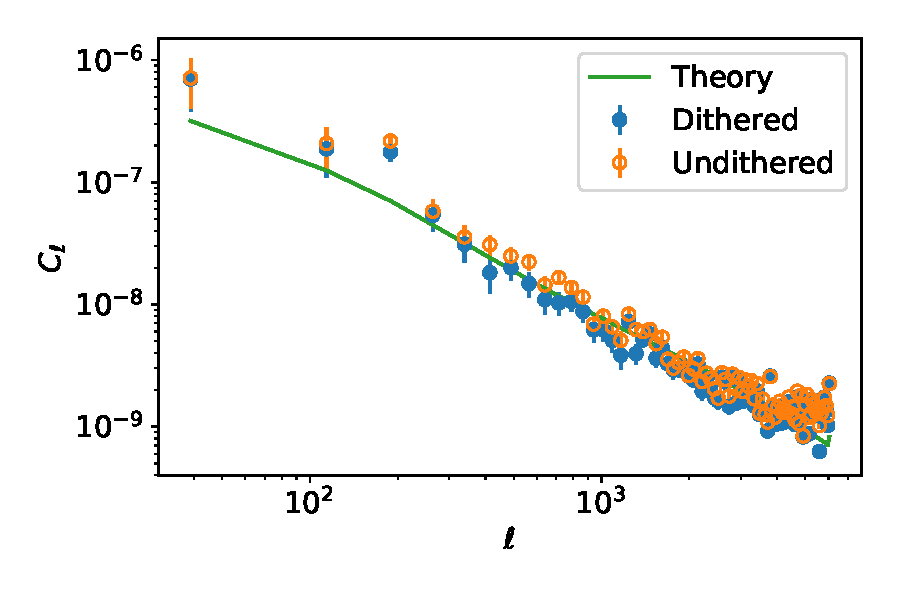
\includegraphics[width=0.9\columnwidth]{Cl_25p3_errors}
\caption{Measured power spectra undithered (open orange circles) and dithered (solid blue circles) datasets with \texttt{NaMaster} corrected by systematics. The error bars are computed using the Gaussian approximation. All datasets seem to be compatible with the theoretical prediction (green line) within 1-$\sigma$.}
\label{fig:power_spectra}
\end{figure}
\subsubsection{Systematic effects}
In this section we analyze the different systematic effects affecting the DC1 data. We will consider the following observational quantities as sources for systematic uncertainties:
\begin{itemize}
\item Extinction: The CatSim catalog provides the value for the magnitudes already corrected for extinction using the SFD map~\citep{1998ApJ...500..525S}. We use this map to cross-correlate with our galaxy catalogs.
\item Stellar contamination: In this case we just build a HEALPix map using the input CatSim stellar catalog to cross-correlate with our galaxy catalogs.
\item Sky-background: We use the observed background level in each exposure and assign that value to the HEALPixel with $N_{side}=2048$ that corresponds to the pointing position. After this we calculate the median value in each HEALPixel and use them to compute the cross-correlations with the galaxy catalogs. The caveat of this approach is that we are not propagating the geometry of the focal plane.
\item Sky-noise: We use the observed noise background level in each exposure and proceed as in the previous case to build a HEALPix map with which we will cross-correlate.
\item Seeing: We proceed as before and use the observed seeing in each exposure and build a HEALPix map.
\end{itemize}
These maps are shown in \figref{systematic_maps} and \figref{systematic_maps2}. 

In the case of the real space measurements, we proceed the same way as ref.~\citep{2016MNRAS.455.4301C} to compute the impact of the different potential sources for systematic uncertainty. We compute the auto and cross-correlations of these maps and our data samples to obtain the ``true`` correlation function:
\begin{equation}
w^{gg}(\theta)_{true} =w^{gg}(\theta)_{obs} -  \vec{w}_{g,sys} \cdot W_{sys,sys}^{-1} \cdot \vec{w}_{g,sys}
\end{equation}
Where $w^{gg}_{true}$ is the corrected galaxy-galaxy correlation function, $w^{gg}_{obs}$ is the measured galaxy-galaxy autocorrelation, $\vec{w}_{g,sys}$ is the vector containing the cross-correlation between the galaxies and the different maps and $W_{sys,sys}^{-1}$ is the inverse of the matrix containing the cross-correlations between different systematics. For the stellar contamination we also follow the procedure presented in ref.~\citep{2016MNRAS.455.4301C}. Given a stellar fraction $f_{star}$ the ``true`` galaxy correlation function is given by
\begin{equation}
w_{gal} = \left(1+f_{star}\right)^{2}\left(w_{obs} - f_{star}^{2}w_{sg} - \frac{f_{star}^{4}}{\left(1+f_{star}\right)^{2}}\right)
\end{equation}
where $w_{sg}$ is the cross-correlation between our stellar map and the observed galaxies.

Comparing with the input catalog we select those objects classified as galaxies whose centroids lie within 2 pixels of a star from the input catalog. From those, we select the objects that have a magnitude difference smaller than 30 mmags. Doing this we estimate a stellar contamination of $f_{star}=7.2\%$ in our sample.

We compare the correction term for the different systematics to the measured signal obtaining the results in \figref{sys_realspace}, where we can appreciate that the dithering strategy is working to reduce the impact of the systematics, keeping them under control and at percent level for $\theta < 0.03 degrees$ in this ``small`` area, improving the signal-to-noise in addition to other benefits explored in ref.~\citep{2016ApJ...829...50A}. This is also seen \figref{2pt_corr} where we clearly see that the uncorrected and corrected correlation function for the dithered field are essentially the same.
\begin{figure}
\centering
%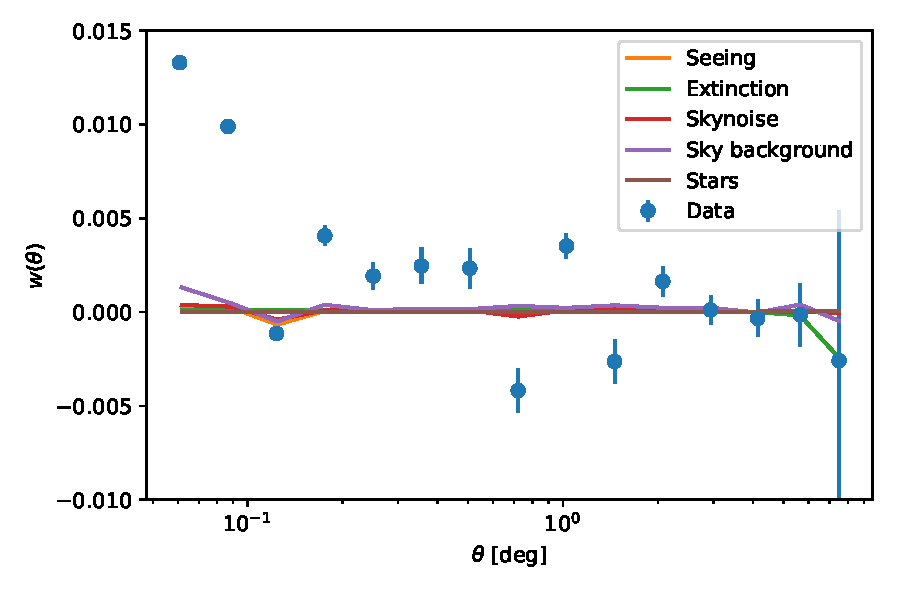
\includegraphics[width=0.9\columnwidth]{w_dithered_25p3.pdf}
%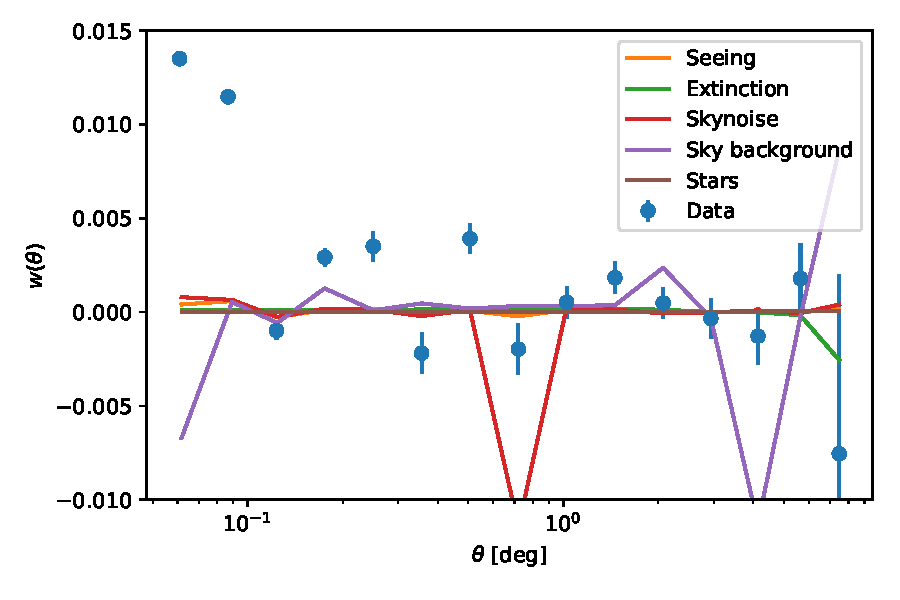
\includegraphics[width=0.9\columnwidth]{w_undithered_25p3.pdf}
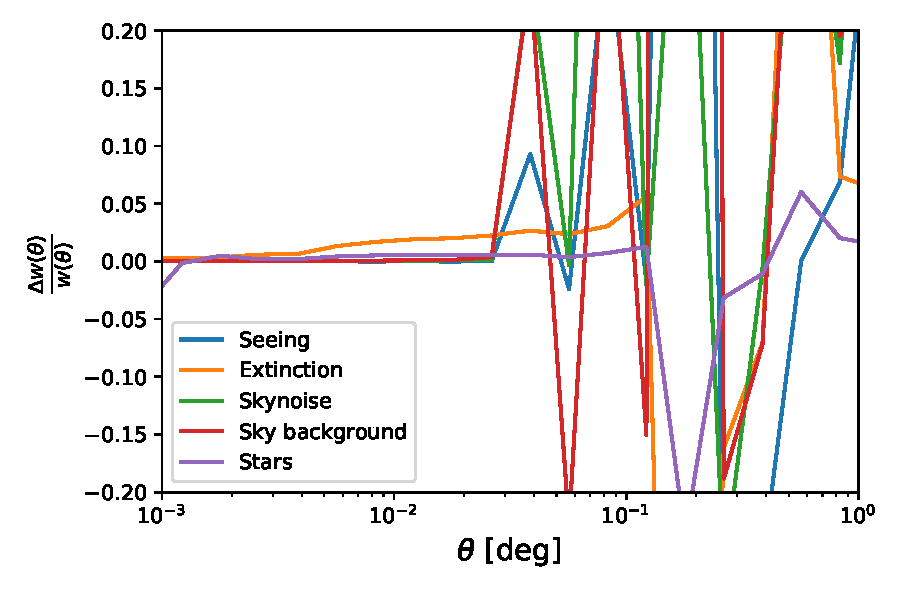
\includegraphics[width=0.9\columnwidth]{sys_dithered_25p3_v2.pdf}
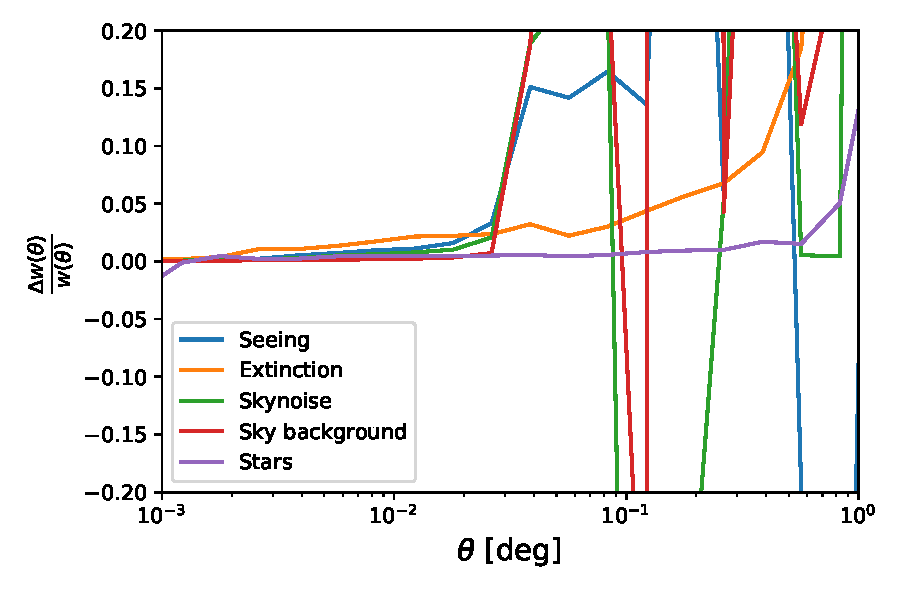
\includegraphics[width=0.9\columnwidth]{sys_undithered_25p3_v2.pdf}
\caption{Correction due to the different potential sources of systematic uncertainty relative to the value of the measured correlation function of the dithered (top) and undithered (bottom) datasets. We show that the correction is at percent level for $\theta<0.03$ degrees and grows beyond the $20\%$ level for $\theta \approx 0.1$ degrees.}
\label{fig:sys_realspace}
\end{figure}

\begin{figure}
\centering
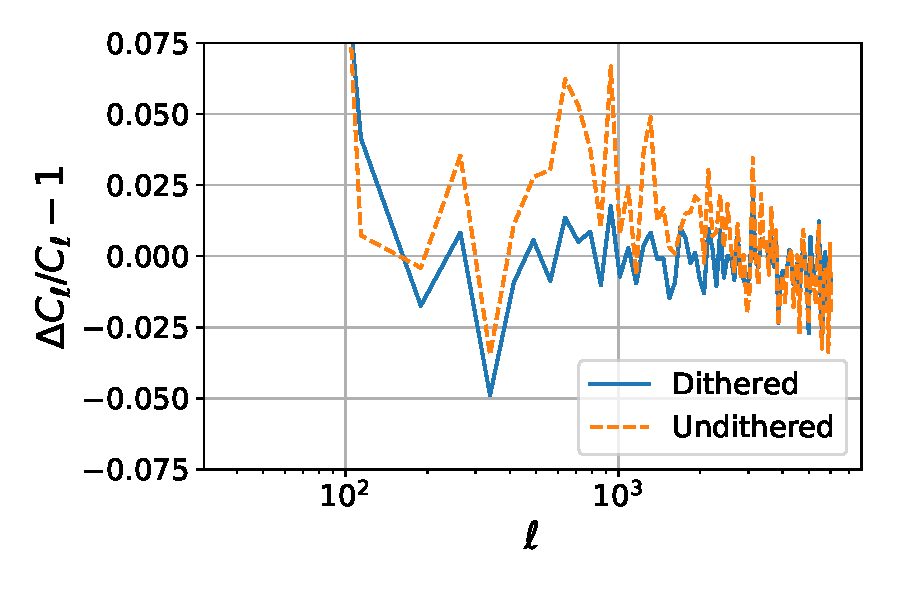
\includegraphics[width=0.9\columnwidth]{Cl_25p3_sys_comparison}
\caption{Correction in harmonic space due to the different potential sources of systematic uncertainty relative to the value of the measured correlation function of the dithered (solid blue) and undithered (dashed orange) datasets.}
\label{fig:sys_harmonic_space}
\end{figure}


In the case of harmonic space we use the mode deprojection from \texttt{NaMaster}~\citep{Namaster} to correct for the different templates. In \figref{sys_harmonic_space} we show the relative size of the correction due to the presence of the considered sources of systematic uncertainty. Again, we see that the dithering strategy diminishes the effect of the potential sources of systematic uncertainty in the power-spectrum measurements.

%\CHECK{Add figure with corrected and uncorrected power-spectra.}

%\subsection{Pushing the dataset further}

%We also wanted to check what happens if we choose a sample where the uniformity across the footprint is still good even though completeness is not as good. We extended our sample by selecting galaxies with \texttt{ $16 < $ CMODEL\_MAG $ < 26.25$} and depth$\geq 26.25$. This increases the sample from 4.3 million galaxies to 6.5 million in the dithered sample, even though the footprint is reduced by $8\%$. However, these selection criteria reduce the number of galaxies to 4.2 million in the undithered sample, as well as the footprint by $35\%$.

\subsection{Reconstructing the selection function}
As we mentioned before, one of the potential applications of this kind of end-to-end studies is the possibility of analyzing how the pipeline performs the data detection and measurement. In terms of the two-point statistics we could think of this as a selection (window) function. In this section we are going to try to reconstruct, to the best of our ability, the selection function given our input and output catalogs.

We will use the spatial matching in \secref{matching} to get the magnitude and the error distribution for our detected galaxies. Then, we bin our sample in 100 true-magnitude bins from 18 to 28, and try to model the difference between input and output flux, $\Delta F$=$F_{meas}$-$F_{true}$, in each bin using a Gaussian mixture model (GMM) with 6 components for objects brighter than 26.4, and 3 components for fainter objects. We chose this threshold since it is close to our faintest $5-\sigma$ limiting magnitude. This way, we have 100 models (one per magnitude bin) to distort the true magnitude and get an emulated magnitude. An example of this GMM can be seen in \figref{example_GMM}. Here we can see that, in a given bin, the GMM captures well the overall distribution of $\Delta F$, so we could potentially estimate the flux error, as a function of magnitude using this model.
\begin{figure}
\centering
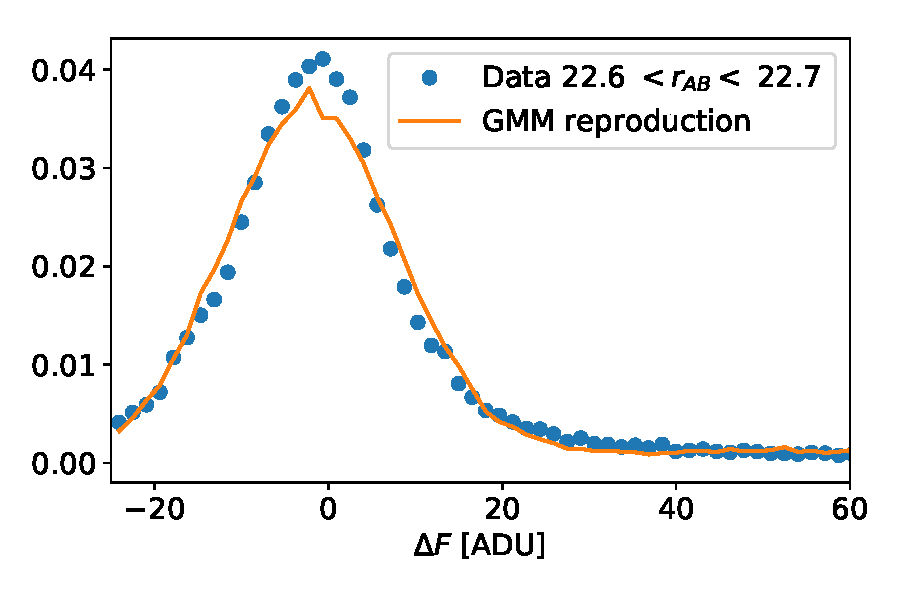
\includegraphics[width=0.9\columnwidth]{example_GMM}
\caption{Measured $\Delta F$ (blue solid circles) compared to 69,000 samples of the Gaussian mixture model that we obtained in the bin $22.6 <$ mag$_{true} < 22.7$. We repeated this for 100 bins between $18 <$ mag$_{true} < 28$.}
\label{fig:example_GMM}
\end{figure}

There are several caveats with this approach: $\Delta F$ is not Gaussian is the center of the distribution is not perfectly described by the GMM regardless of the number of components that we use so our reconstruction will show a slightly larger error than the real data. However, the main problem with this approach is that the models are constructed from detected objects, so the estimated distortions will be biased. When we try to impose some cuts in our emulated magnitudes, we recover a larger number of objects than the detected number. This can be seen in \figref{emulated_magnitudes}, where we used the emulated magnitudes to resemble the selection did for the analyses in previous sections, i.e., we selected objects with $25.3 \geq r_{emulated} \geq 21.4$. In this figure we show the true magnitude distribution for the detected and emulated samples. We see that up to $r _{true} \approx 26$ we have a high level of completeness and our emulation, even though it gives us a larger number of detected objects, makes a good job following the shape of the magnitude distribution. After that, we are dominated by the outliers. This results into a raise of faint emulated objects within our emulated magnitude range. We can also see that, to only use the objects with true magnitudes between the considered range in measured magnitude, i.e., $25.3 \geq r_{true} \geq 21.4$ will result also in a bias in the measured two-point statistics, given that in that case we would be ignoring the (heavy) tails of the magnitude distribution.
\begin{figure}
\centering
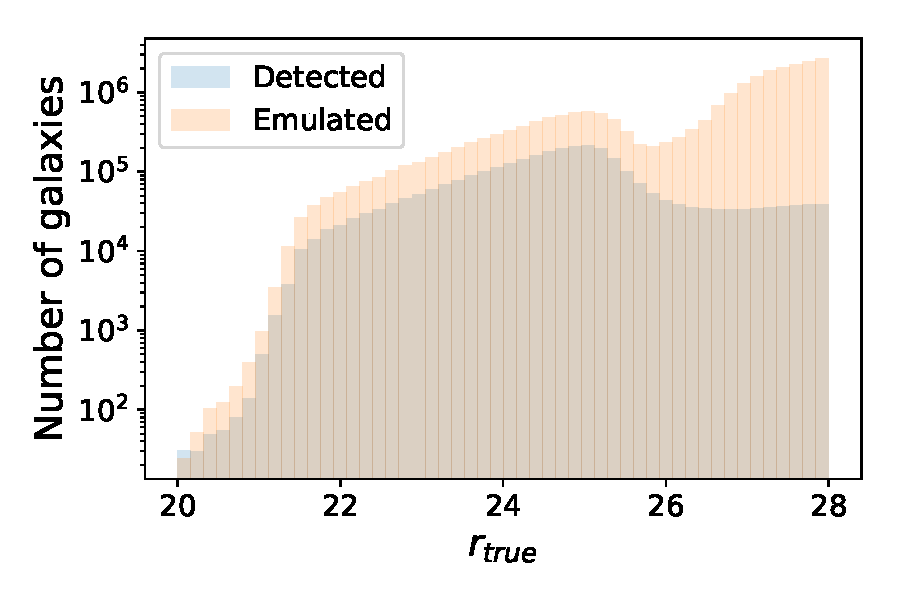
\includegraphics[width=0.9\columnwidth]{emulated_magnitude_histogram}
\caption{True magnitude distribution for the detected objects using spatial matching (blue) and for the emulated objects using the same cuts in measured and emulated magnitude, $25.3 \geq r \geq 21.4$}
\label{fig:emulated_magnitudes}
\end{figure}
This has a noticeable effect in the estimated power-spectra as we can see in \figref{emulated_power}. The power-spectrum using the true magnitude cuts is very close to the  power-spectrum of the detected objects. However, it is smaller than the power-spectrum of the detected objects at small scales. This is likely due to the presence of fainter objects in the latter that are correlated with them. In addition, blended objects can create a small contribution at these scales. Finally, the larger shot-noise can make that the residuals at small scales are larger. On the other hand, at large scales, the power-spectrum using the true magnitude cuts is slightly larger due to the smaller magnitude range (and likely redshift range) considered. On the other hand, we see that the power-spectrum for the emulated magnitude cuts is noticeably lower than the one for the detected objects. This is due to the larger magnitude range considered (so we are averaging over a bigger volume in general). It is clear that this procedure is not good to emulate the selection function of our pipeline, especially given the expected number density of LSST. We also see that just performing cuts on the true magnitude distribution is not enough to recover the measured power-spectrum at the level of precision that we will have with LSST data. Therefore, more sophisticated ways of emulating the processing pipeline should be implemented, and tools like \texttt{BALROG}~\citep{2016MNRAS.457..786S}, \texttt{imSim}, or \texttt{PhoSim}~\citep{2015ApJS..218...14P} that generate synthetic images applied to random (zero-power-spectra) catalogs are interesting for future studies, and achieving percent-level sensitivities.
\begin{figure}
\centering
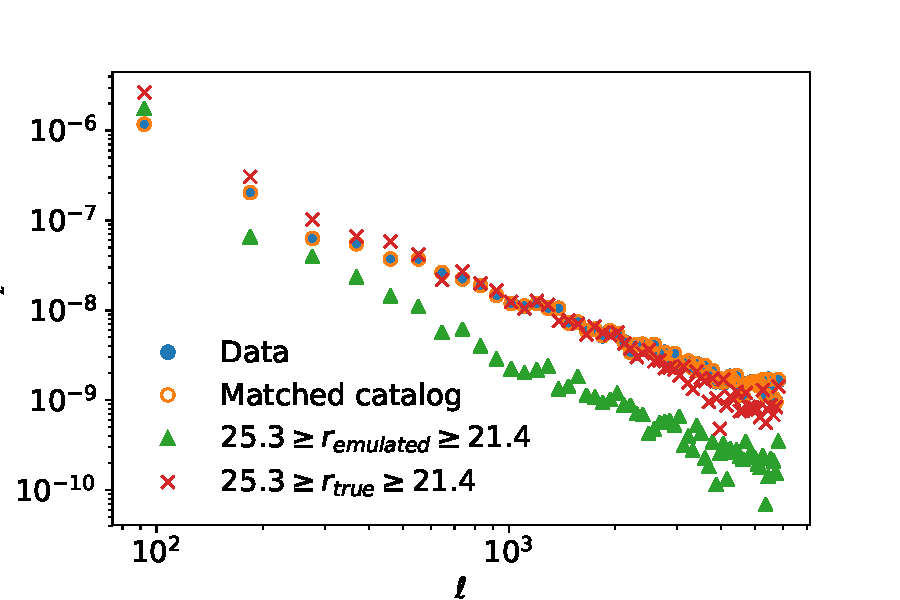
\includegraphics[width=0.9\columnwidth]{emulated_power_spectra}
\caption{Shot-noise subtracted measured power-spectra for the detected objects by the LSST tack (solid blue circles), the objects in the true catalog spatially matched (open orange circles), the objects with $21.4 \leq r_{true} \leq 25.3$ (red crosses), and the objects with $21.4 \leq r_{emulated} \leq 25.3$ (green triangles).}
\label{fig:emulated_power}
\end{figure}
% ----------------------------------------------------------------------

\section{Conclusions}
\label{sec:conclusions}

End-to-end simulations are very useful tools to test the overall performance of any current and future cosmological experiments like the LSST~\citep{2008arXiv0805.2366I}. They allow us to test and improve different parts involved in the data processing and analysis. On the other hand, they also allow us to model and improve our control of systematic uncertainties.

In this paper we have presented a simulated (end-to-end) imaging dataset to resemble LSST data, corresponding to the first data challenge in LSST DESC. We simulated images using state of the art tools (\textit{imSim}). We generated two different and complementary datasets, one with random dithers (\textit{dithered}) and the other with no dithering (\textit{undithered}). Then we processed these images with the LSST DM stack. We started by performing several quality assurance tests on the outputs from the DM stack, including photometry and astrometry checks. We checked that both the \textit{dithered} and \textit{undithered} are high-quality datasets with good photometry and astrometry (with the caveat of uncorrected proper motion). 

After this, we studied different ways to relate the output catalogs to the inputs. In particular, we analyzed spatial matching, and spatial matching including magnitude matching. We saw that the angular power-spectrum is recovered at a very high-level of precision for both cases, however, these matching techniques are likely not good enough for studies about blending or very small scale information. One of the main advantages of the end-to-end simulations is that photons can be traced back to the original sources, however, this is not always possible due different factors such as, data volume limitations so, an important topic for these kind of end-to-end simulations will be to find efficient strategies to relate inputs and outputs.
 
Finally, we estimated the depth and selected a high-completeness sample to perform clustering analysis, in both real and harmonic space. The results of this analysis, indicate that the simulated foregrounds have a low impact at the scales considered for our study (lower than $5\%$ for $\theta < 0.03^{\circ}$ and for the $\ell$ range studied in harmonic space) especially, in the \textit{dithered} dataset. This indicates the success of the dithering strategy considered in this study. We also made a pilot study to try to reconstruct the selection function of our pipeline. We noticed that simple methods cannot capture the complexity of our data given the high sensitivity that we will have in LSST and concluded that more complex methods should be studied in order to perform this operation.

The methodology presented here will serve as basis for future DESC data challenges. In this future data challenges, we aim to perform multi-band studies in a larger area, analyze complementary image generation strategies (\texttt{PhoSim}), increase the complexity of the foregrounds included.

% ----------------------------------------------------------------------

\subsection*{Acknowledgments}

This research used resources of the National Energy Research Scientific Computing Center, a DOE Office of Science User Facility supported by the Office of Science of the U.S. Department of Energy under Contract No. DE-AC02-05CH11231. We acknowledge the use of \texttt{Pandas, Dask, SciPy, Matplotlib, Jupyter, CCL, NaMaster, Healpy, and scikit-learn} as well as the LSST software stack.

%
The DESC acknowledges ongoing support from the Institut National de Physique Nucl\'eaire et de Physique des Particules in France; the Science \& Technology Facilities Council in the United Kingdom; and the Department of Energy, the National Science Foundation, and the LSST Corporation in the United States.  DESC uses resources of the IN2P3 Computing Center (CC-IN2P3--Lyon/Villeurbanne - France) funded by the Centre National de la Recherche Scientifique; the National Energy Research Scientific Computing Center, a DOE Office of Science User Facility supported by the Office of Science of the U.S.\ Department of Energy under Contract No.\ DE-AC02-05CH11231; STFC DiRAC HPC Facilities, funded by UK BIS National E-infrastructure capital grants; and the UK particle physics grid, supported by the GridPP Collaboration.  This work was performed in part under DOE Contract DE-AC02-76SF00515.
This manuscript has been authored by Fermi Research Alliance, LLC under Contract No. DE-AC02-07CH11359 with the U.S. Department of Energy, Office of Science, Office of High Energy Physics.

% 


%{\it Facilities:} \facility{LSST}

% Include both collaboration papers and external citations:
\bibliography{lsstdesc,main}

\appendix
\section{Mapping observational effects}
\label{sec:systematic_maps}
\begin{figure}
\centering
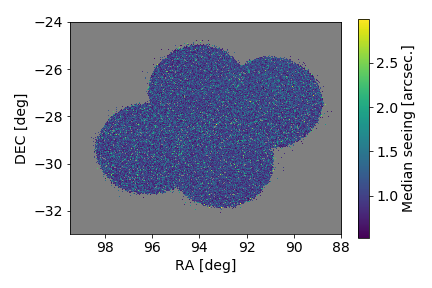
\includegraphics[width=0.7\columnwidth]{median_seeing.png}
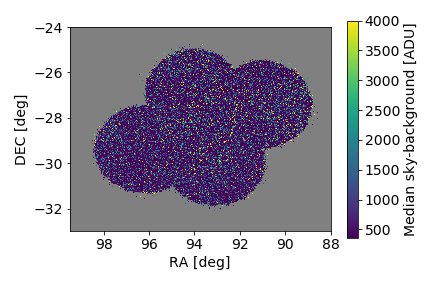
\includegraphics[width=0.7\columnwidth]{median_skybg.png}
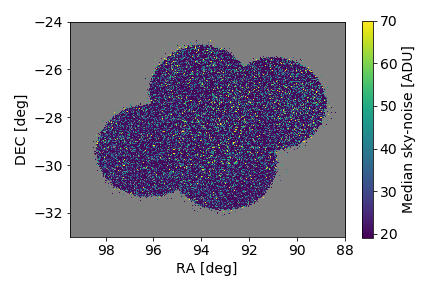
\includegraphics[width=0.7\columnwidth]{median_skynoise.png}
\caption{HEALPix maps showing the different observational effects that might be potential cause of systematic uncertanties.}
\label{fig:systematic_maps}
\end{figure}
\begin{figure}
\centering
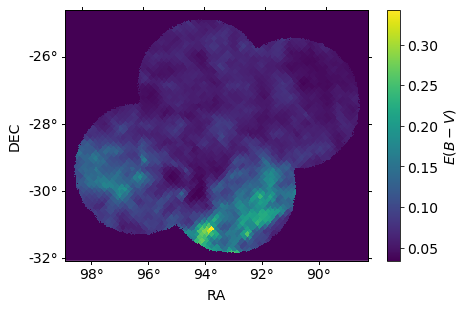
\includegraphics[width=0.7\columnwidth]{extinction.png}
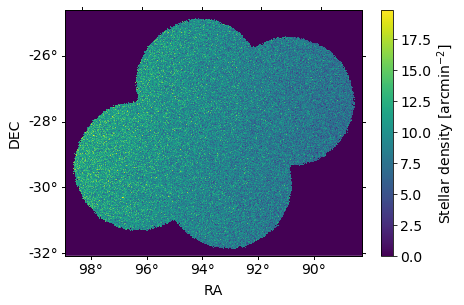
\includegraphics[width=0.7\columnwidth]{stellar_density.png}
\caption{HEALPix maps showing the different observational effects that might be potential cause of systematic uncertanties.}
\label{fig:systematic_maps2}
\end{figure}
\end{document}
% ======================================================================
%
